% -*- LaTeX -*-

% PLEASE USE THIS FILE AS A TEMPLATE FOR THE DOCUMENTATION OF YOUR OWN
% FACILITIES: IN PARTICULAR, IT IS IMPORTANT TO NOTE COMMENTS MADE IN
% THE TEXT AND TO FOLLOW THIS ORDERING. THE FORMAT FOLLOWS ONE USED BY
% THE COBE-DMR PROJECT.	
% A.J. Banday, April 1999.

\documentclass[12pt,twoside]{article}
%\usepackage{xr-hyper,healpix,html,makeidx,tabularx} 
%%\usepackage{xr-hyper,healpix,html,makeidx} 
\usepackage{xr-hyper,healpix,graphicx,html,makeidx} 
%\usepackage{healpix,xr-hyper,html,graphicx,makeidx}
\usepackage{ae,lmodern}% load vectorial font, keep PDF small *and* good quality when in T1 font
\usepackage[T1]{fontenc}% underscore searchable in PDF, but larger PDF http://latex-community.org/forum/viewtopic.php?t=8891
\begin{htmlonly}
% \renewcommand{\backslash}{\}
% \renewcommand{\ell}{l} % not necessary with 2018's latex2html
 \renewcommand{\lq}{'}
 % -*- LaTeX -*-
% This LaTeX file sets the Healpix version
% as it will appear in the documentation
% implement it with: % -*- LaTeX -*-
% This LaTeX file sets the Healpix version
% as it will appear in the documentation
% implement it with: % -*- LaTeX -*-
% This LaTeX file sets the Healpix version
% as it will appear in the documentation
% implement it with: \input{hpxversion}
% \newcommand{\hpxversion}{3.31}
% \newcommand{\hpxverstex}{3\_31}
% \newcommand{\hpxversion}{3.40}
% \newcommand{\hpxverstex}{3\_40}
% \newcommand{\hpxversion}{3.41}
% \newcommand{\hpxverstex}{3\_41}
\newcommand{\hpxversion}{3.50}
\newcommand{\hpxverstex}{3\_50}

% \newcommand{\hpxversion}{3.31}
% \newcommand{\hpxverstex}{3\_31}
% \newcommand{\hpxversion}{3.40}
% \newcommand{\hpxverstex}{3\_40}
% \newcommand{\hpxversion}{3.41}
% \newcommand{\hpxverstex}{3\_41}
\newcommand{\hpxversion}{3.50}
\newcommand{\hpxverstex}{3\_50}

% \newcommand{\hpxversion}{3.31}
% \newcommand{\hpxverstex}{3\_31}
% \newcommand{\hpxversion}{3.40}
% \newcommand{\hpxverstex}{3\_40}
% \newcommand{\hpxversion}{3.41}
% \newcommand{\hpxverstex}{3\_41}
\newcommand{\hpxversion}{3.50}
\newcommand{\hpxverstex}{3\_50}

 % -*- LaTeX -*-
% This LaTeX file sets the Healpix websites
% as they will appear in the documentation
% implement it with: % -*- LaTeX -*-
% This LaTeX file sets the Healpix websites
% as they will appear in the documentation
% implement it with: % -*- LaTeX -*-
% This LaTeX file sets the Healpix websites
% as they will appear in the documentation
% implement it with: \input{hpxwebsites}

% -------- mailing list
\newcommand{\healpixmail}{{\em healpix-support} \texttt{at} {\em lists.sourceforge.net}}

% -------- source web site: see healpix_src_url.tex

% -------- doc web site
\newcommand{\hpxwebsite}{https://healpix.sourceforge.io}
\newcommand{\oldhpxwebsite}{http://healpix.sf.net}

% --------- used in install.tex:
%\newcommand{\healpixwebpage}{\oldhpxwebsite}
\newcommand{\healpixwebpage}{\hpxwebsite}
\newcommand{\healpixsupport}{\healpixwebpage/support.php}

% DO NOT FORGET TO UPDATE main.html AS WELL !!!!!


%--------------------- web site(s) showing on front page
% %OLD
% \newcommand{\defwebsite}{\website{\htmladdnormallink{\oldhpxwebsite}{\oldhpxwebsite}}}

%TRANSITION
\newcommand{\defwebsite}{\website{\htmladdnormallink{\hpxwebsite}{\hpxwebsite}\\\htmladdnormallink{\oldhpxwebsite}{\oldhpxwebsite}}}

% %FUTURE
% \newcommand{\defwebsite}{\website{\htmladdnormallink{\hpxwebsite}{\hpxwebsite}}}




% -------- mailing list
\newcommand{\healpixmail}{{\em healpix-support} \texttt{at} {\em lists.sourceforge.net}}

% -------- source web site: see healpix_src_url.tex

% -------- doc web site
\newcommand{\hpxwebsite}{https://healpix.sourceforge.io}
\newcommand{\oldhpxwebsite}{http://healpix.sf.net}

% --------- used in install.tex:
%\newcommand{\healpixwebpage}{\oldhpxwebsite}
\newcommand{\healpixwebpage}{\hpxwebsite}
\newcommand{\healpixsupport}{\healpixwebpage/support.php}

% DO NOT FORGET TO UPDATE main.html AS WELL !!!!!


%--------------------- web site(s) showing on front page
% %OLD
% \newcommand{\defwebsite}{\website{\htmladdnormallink{\oldhpxwebsite}{\oldhpxwebsite}}}

%TRANSITION
\newcommand{\defwebsite}{\website{\htmladdnormallink{\hpxwebsite}{\hpxwebsite}\\\htmladdnormallink{\oldhpxwebsite}{\oldhpxwebsite}}}

% %FUTURE
% \newcommand{\defwebsite}{\website{\htmladdnormallink{\hpxwebsite}{\hpxwebsite}}}




% -------- mailing list
\newcommand{\healpixmail}{{\em healpix-support} \texttt{at} {\em lists.sourceforge.net}}

% -------- source web site: see healpix_src_url.tex

% -------- doc web site
\newcommand{\hpxwebsite}{https://healpix.sourceforge.io}
\newcommand{\oldhpxwebsite}{http://healpix.sf.net}

% --------- used in install.tex:
%\newcommand{\healpixwebpage}{\oldhpxwebsite}
\newcommand{\healpixwebpage}{\hpxwebsite}
\newcommand{\healpixsupport}{\healpixwebpage/support.php}

% DO NOT FORGET TO UPDATE main.html AS WELL !!!!!


%--------------------- web site(s) showing on front page
% %OLD
% \newcommand{\defwebsite}{\website{\htmladdnormallink{\oldhpxwebsite}{\oldhpxwebsite}}}

%TRANSITION
\newcommand{\defwebsite}{\website{\htmladdnormallink{\hpxwebsite}{\hpxwebsite}\\\htmladdnormallink{\oldhpxwebsite}{\oldhpxwebsite}}}

% %FUTURE
% \newcommand{\defwebsite}{\website{\htmladdnormallink{\hpxwebsite}{\hpxwebsite}}}



\end{htmlonly}

\hypersetup{%
	pdftitle={HEALPix Fortran Facilities Overview},%
	pdfauthor={E. Hivon et al},%
	pdfkeywords={HEALPix, Fortran},%
	colorlinks=true}%

\newcommand{\nside}{N_{\mathrm{side}}}
\newcommand{\npix}{N_{\mathrm{pix}}}
\newcommand{\lmax}{\ell_{\mathrm{max}}}
%\newcommand{\myhtmlimage}[1]{\htmlimage{#1}}
\newcommand{\myhtmlimage}[1]{ }
\renewcommand{\contentsname}{{TABLE OF CONTENTS}}

% command for external link
\newcommand{\linklatexhtml}[3]{% \linklatexhtml{name}{latex_target}{html_target}
\latexhtml{\htmladdnormallink{#1}{#2}}{\htmladdnormallink{#1}{#3}}}
% commands for arbitrary link
\newcommand{\mylink}[2]{% \mylink{link_id}{link_text}
\latexhtml{\hyperlink{#1}{#2}}{\hyperref{#2}{}{}{#1}}}
\newcommand{\mylinkext}[2]{% \mylink{link_id}{link_text}  (external link)
\latexhtml{\htmlref{#2}{#1}}{\hyperref{#2}{}{}{#1}}}
% commands for targets 
% http://tex.stackexchange.com/questions/17057/hypertarget-seems-to-aim-a-line-too-low
\makeatletter
     \newcommand{\nop}[1]{\Hy@raisedlink{\hypertarget{#1}{}}}
\makeatother
\newcommand{\mytarget}[1]{\nop{#1}\phantomsection\label{#1}}%    \mytarget{id}
%\newcommand{\mytarget}[1]{\nop{#1}}%    \mytarget{id}
\begin{htmlonly}
 \newcommand{\mytarget}[1]{\label{#1}}
\end{htmlonly}
\newcommand{\doubledash}{\latexhtml{-{}-}{-{}--}} %used in install.pdf

% macros for old changes
\newcommand{\mysmaller}{% small in LaTeX, normal in html
\latexhtml{\scriptsize}{\normalsize}}
\newcommand{\compresstext}{% smaller vertical spacing in LaTeX, normal in html
\latexhtml{%
\setlength{\parsep}{-3ex}%
\setlength{\topsep}{0ex}%
\setlength{\parskip}{0ex}}{}}
\newcommand{\compresslist}{% smaller vertical spacing in list in LaTeX, normal in html
\setlength{\itemsep}{0ex}}{}

\sloppy
\setcounter{secnumdepth}{0}
\setcounter{tocdepth}{1}


% CROSS-LINK
%%%%http://tex.stackexchange.com/questions/41539/does-hyperref-work-between-two-files
%% add xr-hyper (part of hyperref) to used packages, *BEFORE* hyperref (or html)
\newcommand{\facname}{} % must be here because it is in idl.tex
\newcommand{\FACNAME}{} % must be here because it is in idl.tex
\externaldocument{intro}[intro.pdf]
\externaldocument{install}[install.pdf]
\externaldocument{csub}[csub.pdf]
\externaldocument{idl}[idl.pdf]
%\externaldocument{facilities}[facilities.pdf]
\externaldocument{subroutines}[subroutines.pdf]
\begin{htmlonly}
\externallabels{.}{/tmp/introlabels.pl}
\externallabels{.}{/tmp/intro_labels.pl}
\externallabels{.}{/tmp/installlabels.pl}
\externallabels{.}{/tmp/install_labels.pl}
\externallabels{.}{/tmp/csublabels.pl}
\externallabels{.}{/tmp/csub_labels.pl}
\externallabels{.}{/tmp/idllabels.pl}
\externallabels{.}{/tmp/idl_labels.pl}
%\externallabels{.}{/tmp/facilitieslabels.pl}
%\externallabels{.}{/tmp/fac_labels.pl}
\externallabels{.}{/tmp/subroutineslabels.pl}
\externallabels{.}{/tmp/sub_labels.pl}
\end{htmlonly}

% \newcommand{\aboutoptional}{Arguments appearing in \optional{italic} are
% optional.}
% \newcommand{\modHeadFits}{src/f90/mod/head\_fits.F90}

%%%%%
\begin{document}
\title{\healpix Fortran Facility User Guidelines}
\label{fac:facilities}
\docrv{Version \hpxversion}
\author{Eric Hivon, Frode K.~Hansen, Benjamin D.~Wandelt, Krzysztof M.~G\'orski,
Anthony J.~Banday, Martin Reinecke}
\abstract{This document describes the \healpix Fortran stand-alone facilities}
%% -*- LaTeX -*-
% This LaTeX file sets the Healpix website
% as it will appear in the documentation
% implement it with: % -*- LaTeX -*-
% This LaTeX file sets the Healpix website
% as it will appear in the documentation
% implement it with: % -*- LaTeX -*-
% This LaTeX file sets the Healpix website
% as it will appear in the documentation
% implement it with: \input{hpxwebsite}
%
% DEPRECATED !!!! replaced with hpxwebsites.tex
%

%
% DEPRECATED !!!! replaced with hpxwebsites.tex
%

%
% DEPRECATED !!!! replaced with hpxwebsites.tex
%

\defwebsite
\date{\today}

\frontpage
%\newpage
\tableofcontents
\newpage

\section{Using the \healpix Fortran 90 facilities}
% {\bf {Default File Names and Directories}}: 
\subsection{Default file names and directories}
\label{fac:subsec:defdir}
For some applications, the \healpix facilities
require some precalculated input files describing the pixel window
function and ring-based or pixel-based quadrature weights (shipped as 
{\tt Healpix/data/pixel\_\-window\_\-n????.fits},
{\tt Healpix/data/weight\_\-ring\_\-n?????.fits} and
{\tt Healpix/data/weight\_\-pixel\_\-n?????.fits} respectively). \label{page:defdir}

By default, files with the very same name (generated by functions such as 
\htmlref{\texttt{get\_\-healpix\_\-pixel\_\-window\_\-file}}{sub:get_healpix_xxx_file}) 
will be looked for into a list of directories (generated by 
\htmlref{\texttt{get\_\-healpix\_\-data\_\-dir}}{sub:get_healpix_xxx_dir}) 
containing the current directory (\texttt{.}), the parent directory (\texttt{..}),
\texttt{./data}, \texttt{../data}, \texttt{\$HEALPIX} and \texttt{\$HEALPIX/data} where \texttt{\$HEALPIX} is
a system variable defined as the full path to the \healpix package
(see the installation documentation).\\
However, the user has the possibility to change both the name of those files
and their location (with options like 
\texttt{windowfile},
\texttt{winfiledir},
\texttt{w8file}, or
\texttt{w8filedir})

%% \vskip 1cm
%% {\bf {Input and Output Precision}}: several facilities offer the option of
%% changing the input and output data arrays from single to double precision
%% floating point reals. The following points should be noted: \label{page:ioprec}
%% \begin{itemize}
%% \item Double precision IO facilities can read indifferently single and double
%%   precision data files (and the same is true for single precision facilities). On
%%   the other hand, a double (resp. single) precision facility will only output double
%%   (single) precision  files.
%% \item Since the internal calculations sensitive to numerical round-off error
%%   (like the spherical harmonics recurrence) are
%%   {\em always} performed in double precision, switching to double precision IO
%% \begin{itemize}
%% \item   will have a limited impact on the output accuracy if the input file contains
%%   single precision data,
%% \item is recommended if the input file contains double precision data,
%% \item will not alter the execution speed, but
%%   it will almost double the memory consumption.
%% \end{itemize}
%% \end{itemize}
% \vskip 1cm
% {\bf {Double/Single Precision mode}}: s
\subsection{Double/Single precision mode}
\label{fac:subsec:ioprec}
Several facilities offer the option of switching at run time 
the precision of the internal variables and arrays and of the I/O data from single to double precision
floating point reals. The following points should be noted: \label{page:ioprec}
\begin{itemize}
\item Facilities running in double precision mode can read indifferently single and double
  precision data files (and the same is true for single precision facilities). On
  the other hand, a double (resp. single) precision facility will only output double
  (single) precision  files.
\item Since the internal calculations sensitive to numerical round-off error
  (like the spherical harmonics recurrence) are
  {\em always} performed in double precision, switching to double precision mode
\begin{itemize}
\item   will have a limited impact on the output accuracy if the input file contains only
  single precision data,
\item is recommended if the input file contains double precision data, and the precision of the output is critical
\item will only increase a bit the execution time (by 15\% in some of our tests), but
  it will almost double the memory consumption of the facility,
\item will obviously double the size of the output file(s).
\end{itemize}
\end{itemize}

%\vskip 1cm
\subsection{Beam window function files}
\label{fac:subsec:beamfiles}
%Beam window function files.
Several F90 and IDL applications (eg,
\htmlref{\tt alteralm}{fac:alteralm}, 
\htmlref{\tt sky\_ng\_sim}{fac:sky_ng_sim}, 
\htmlref{\tt smoothing}{fac:smoothing}, 
\htmlref{\tt synfast}{fac:synfast}, 
\htmlref{\tt ialteralm}{idl:ialteralm}, 
\htmlref{\tt ismoothing}{idl:ismoothing}, 
\htmlref{\tt isynfast}{idl:isynfast})
accept, generally with the argument {\tt beam\_file} a circular (possibly non-gaussian) beam or smoothing window,
which is described under the form of its {\em real} (polarized) Legendre window functions
(see IDL's \htmlref{\tt beam2bl}{idl:beam2bl})
read from an external file.\label{page:beamfiles}
The file is either 
\begin{itemize}
\item 
{\em highly recommended:} a FITS file containing a binary or ASCII table, with 1, 2 or 3 fields, respectively\\
$b_T(\ell)$, [$b_E(\ell)$, [$b_B(\ell)$]]
\item 
 in IDL, is can also be an array of size ($\lmax+1$,$d$) with $d=$1, 2 or 3, which will be 
automatically turned into a FITS file of the format described above using the 
\healpixns/IDL routine \htmlref{\tt bl2fits}{idl:bl2fits}.
\item 
or, it can also be, a plain text file with 2, 3 or 4 columns, containing, on each line,  \\
$\ell$, $b_T(\ell)$, [$b_E(\ell)$, [$b_B(\ell)$]]\\ 
and in which lines starting with a \# sign are ignored.
\end{itemize}
In any case, 
the multipole $\ell$ must take all integer values in $\{0,\ldots,\lmax\}$, 
with the assumption that the window functions vanish outside that range.
$b_T$ is the 'temperature' or intensity window function, 
while the optional $b_E$ and $b_B$ are respectively the electric (or gradient) and
magnetic (or curl) components of polarization.
If not provided, $b_B(\ell)$ takes the value of $b_E(\ell)$ which itself defaults to $b_T(\ell)$.
With these window functions, the (polarized) 
map spherical harmonics coefficients and its power spectra are transformed according to
\begin{eqnarray}
	a^{X}_{\ell m} &\longrightarrow& a^{X}_{\ell m} b_{X}(\ell),\\
	C^{XY}_{\ell m} &\longrightarrow& C^{XY}_{\ell m} b_{X}(\ell)b_{Y}(\ell),
\end{eqnarray}
with $X,Y \in \{T,E,B\}$.

\newpage

%--------------------------------------------
%-------------------------------------------- CHANGES
%--------------------------------------------
\section[Changes between releases 3.60 and \hpxversion]{%
Changes between releases 3.60 and \hpxversion}
\begin{itemize}
\item Addition of the subroutines
\mylinkext{sub:read_fits_partial}{\texttt{read\_fits\_partial}},
and 
\mylinkext{sub:write_fits_partial}{\texttt{write\_fits\_partial}},
to read and write
polarized or unpolarized map defined on a fraction of the sky.
\end{itemize}

%--------------------------------------------
\section[Older Changes]{Older Changes}
%--------------------------------------------

%%%%{\footnotesize{%
{\mysmaller%
\compresstext
%
\subsubsection{Version 3.60}
\begin{itemize}
\item Faster Spherical Harmonics Transforms 
in 
\htmlref{\texttt{anafast}}{fac:anafast},
\htmlref{\texttt{smoothing}}{fac:smoothing},
and \htmlref{\texttt{synfast}}{fac:synfast}
thanks to the \htmlref{new \texttt{libsharp} library}{install:libsharp:config}.
\end{itemize}
%
%-------------------------
\subsubsection{Version 3.50}
\begin{itemize}
%
% \item correction of a bug in \mylinkext{sub:map2alm_iterative}{\texttt{map2alm\_iterative}}
% when a \mylinkext{sub:map2alm_iterative:mask}{\texttt{mask}} is used in combination with 
% \mylinkext{sub:map2alm_iterative:iter_order}{\texttt{iter\_order}} $> 0$,
\item correction of a bug in \htmlref{\texttt{anafast}}{fac:anafast} when
\mylink{fac:anafast:maskfile}{\texttt{maskfile}} or 
\mylink{fac:anafast:theta_cut_deg}{\texttt{theta\_cut\_deg}}
are used in combination with 
\mylink{fac:anafast:iter_order}{\texttt{iter\_order}}$>0$,
%
\item addition of \mylinkext{sub:alm2map:zbounds}{\texttt{zbounds}} in 
\mylinkext{sub:alm2map}{\texttt{alm2map}},
\mylinkext{sub:alm2map_der}{\texttt{alm2map\_der}},
\mylinkext{sub:alm2map_spin}{\texttt{alm2map\_spin}},
in order to simulate (faster) a signal on only a fraction of the sphere,
%
\item  \htmladdnormallink{improved support for version 18 and more of Intel C and F90 compilers}{https://sourceforge.net/p/healpix/bugs/78} in \texttt{configure} script,
%
\item \htmladdnormallink{edition to fitstools.F90}{https://sourceforge.net/p/healpix/bugs/84} allowing a proper compilation with g95.
\end{itemize}


%-------------------------
\subsubsection{Version 3.40}
% \section[Changes between releases 3.31 and 3.40]{%
% Changes between releases 3.31 and 3.40}

%from install.tex
\begin{itemize}\compresslist
\item The facilities 
\htmlref{\texttt{anafast}}{fac:anafast} and 
\htmlref{\texttt{smoothing}}{fac:smoothing} now support pixel-based quadrature weights.
Introduction of the supporting 
\htmlref{\texttt{nside2npweights}}{sub:nside2npweights},
\htmlref{\texttt{unfold\_weightsfile}}{sub:unfold_weightsfile},
\mylinkext{sub:get_healpix_xxx_file:ghw8f}{\texttt{get\_healpix\_weight\_file}},
\mylinkext{sub:get_healpix_xxx_file:ghpw8f}{\texttt{get\_healpix\_pixel\_weight\_file}}.
%
\item The facilities 
\htmlref{\texttt{anafast}}{fac:anafast},
\htmlref{\texttt{median\_filter}}{fac:median_filter},
\htmlref{\texttt{smoothing}}{fac:smoothing}, and
\htmlref{\texttt{ud\_grade}}{fac:ud_grade} 
test the value of the \texttt{POLCCONV} FITS keyword when reading a polarized map,
and interpret the polarization accordingly, 
as described in the \htmlref{note on POLCCONV}{intro:polcconv} in \linklatexhtml{The \healpix Primer}{intro.pdf}{intro.htm}.
%
\item%
\htmlref{\texttt{median\_filter}}{fac:median_filter} faster by moving an internal array from heap to stack; does not crash anymore when dealing with empty data sets; 
slightly different output when median is computed over an even number of pixels $n\ge 100$, sorted in $[1,n]$,
the output is $d(n/2)$ instead of $(d(n/2)+d(n/2+1))/2$ previously. Result remains $d(n/2+1)$ for odd $n$.
\end{itemize}

%%%%%%

%\setlength{\partopsep}{0}

%-------------------------
\subsubsection{Version 3.31}
\begin{itemize}\compresslist
	\item Bug correction in \htmlref{{\tt input\_map}}{sub:input_map} routine for reading of polarized multi-HDU cut sky FITS files;
	\item Introduction of 
\mylink{fac:alteralm:winfiledir_in}{{\tt winfiledir\_*}} and 
\mylink{fac:alteralm:windowfile_in}{{\tt windowfile\_*}} qualifiers in \htmlref{{\tt alteralm}}{fac:alteralm} facility.
\end{itemize}

%-------------------------
\subsubsection{Version 3.30}
\begin{itemize}\compresslist
	\item \htmlref{{\tt anafast}}{fac:anafast} now produces nine spectra 
	(TT, EE, BB, TE, TB, EB, ET, BT and BE), instead of six previously,
          when analyzing two polarized maps
	\item CFITSIO version 3.20 (August 2009) or more now required
\end{itemize}


% \subsection[Changes between releases 3.00 and 3.20]{%
% Changes between releases 3.00 and 3.20}

%-------------------------
\subsubsection{Version 3.20}
\begin{itemize}\compresslist
	\item \healpixns-F90 routines and facilities can now also be compiled with
the free Fortran95 compiler \textbf{g95} (\htmladdnormallink{www.g95.org}{http://www.g95.org/})
 	\item a separate {\tt build} directory is used to store the objects,
modules, ... produced during the compilation of the source codes
	\item improved handling of long FITS keywords, now producing FITS files
fully compatible with the
\htmladdnormallink{\tt PyFITS}{https://pypi.org/project/pyfits/3.3}
and 
{\tt Astropy} (\htmladdnormallink{https://www.astropy.org}{https://www.astropy.org/})
{\tt Python} libraries
	\item improved FITS file parsing in 
\htmlref{{\tt generate\_beam}}{sub:generate_beam},
affecting the external $B(l)$ reading in the F90 facilities 
\htmlref{{\tt alteralm}}{fac:alteralm}, 
\htmlref{{\tt synfast}}{fac:synfast}, 
\htmlref{{\tt sky\_ng\_sim}}{fac:sky_ng_sim}, 
\htmlref{{\tt smoothing}}{fac:smoothing}.
\end{itemize}

\subsubsection{Version 3.11}
\begin{itemize}\compresslist
	\item {\tt libsharp} C routines used for Spherical Harmonics Transforms 
and introduced in \healpix\ 3.10
can now be compiled with any {\tt gcc} version.
\end{itemize}

\subsubsection{Version 3.10}
\begin{itemize}\compresslist
%
	\item all Fortran facilities now support most of {\tt cfitsio}'s ''\htmladdnormallink{Extended File
Name Syntax}{https://heasarc.gsfc.nasa.gov/docs/software/fitsio/filters.html}'' features,
allowing the reading and processing of an arbitrary HDU and table column out of
remote, compressed FITS files. For example, setting \hfill \\
{\tt infile = }{\tt ftp://}{\it url/file.fits}{\tt .gz}{\tt [}{\it extn}{\tt
]}{\tt [col }{\it colname}{\tt ]}  \hfill \\
in \htmlref{{\tt anafast}}{fac:anafast}
will download the FITS file {\it file.fits.gz} from {\it url}, 
uncompress it, open the HDU (extension) featuring keyword {\tt EXTNAME=}{\it
extn}, or the one with 1-based rank number {\it extn}, read the table column
with {\tt TTYPE*=}{\it colname} out of it and will analyze it.\\
It is also possible to perform a remote \htmlref{{\tt anafast}}{fac:anafast} analysis of a 
%\htmladdnormallink{Planck Legacy Archive (PLA)}{http://www.sciops.esa.int/index.php?project=planck&page=Planck_Legacy_Archive}
\htmladdnormallink{Planck Legacy Archive (PLA)}{https://pla.esac.esa.int/pla/\#home}
sky map named {\it map.fits} via the PLA \htmladdnormallink{AIO Subsystem}%
{https://pla.esac.esa.int/pla/\#aio}
%{http://pla.esac.esa.int/pla/aio/} 
by simply setting
{\tt infile=https://pla.esac.esa.int/pla/aio/product-action?MAP.MAP\_ID=}{\it map.fits}
as input map file.
%
	\item yet faster 
\htmlref{{\tt synfast}}{fac:synfast},
\htmlref{{\tt anafast}}{fac:anafast},
\htmlref{{\tt smoothing}}{fac:smoothing} thanks to \htmladdnormallink{{\tt
libsharp}}{https://sourceforge.net/projects/libsharp} routines\footnote{
To {\em revert} to the original F90 implementation of all these routines, the preprocessing
variable {\tt DONT\_USE\_SHARP} must be set during compilation.}. \\
{\em Note that 
some \htmladdnormallink{{\tt gcc} versions}{https://gcc.gnu.org/releases.html}
(4.4.1 to 4.4.6) crash with an internal compiler error during compilation of {\tt libsharp}}. 
The problem has been fixed in {\tt gcc} 4.4.7, 4.5.*, 4.6.*, 4.7.* and
newer versions and was not present in versions 4.2.* and 4.3.*.
%
\end{itemize}

\subsection[Changes up to release 3.00]{%
Changes up to release 3.00}
\subsubsection{Version 3.00}
\begin{itemize}\compresslist
	\item all {\em input} FITS files can now be compressed (with a 
{\tt .gz}, {\tt .Z}, {\tt .z}, or {\tt .zip} 
extension) and/or remotely located (with a {\tt ftp://} or {\tt http://} prefix).
{\em Version 3.14 (March 2009) or newer of CFITSIO is required for \healpix 3.0.}
	\item introduction of \htmlref{{\tt process\_mask}}{fac:process_mask} 
facility to compute the angular distance of valid
pixels to the closest invalid pixels for a input binary mask,
	\item \htmlref{{\tt sky\_ng\_sim}}{fac:sky_ng_sim} now allows the computation
of the spatial derivatives of the non Gaussian map being produced, and the
output of the $a_{\ell m}$ coefficients of that map,
	\item \htmlref{{\tt anafast}}{fac:anafast} now allows the
pro/down-grading of the input mask to match the resolution of the map(s) being
analyzed.
\end{itemize}


% \subsection[Changes between releases 2.14 and 2.20]{Changes between releases 2.14 and
% 2.20}
\subsubsection{Version 2.20}
\begin{itemize}\compresslist
	\item faster 
\htmlref{{\tt synfast}}{fac:synfast},
\htmlref{{\tt anafast}}{fac:anafast},
\htmlref{{\tt smoothing}}{fac:smoothing} thanks to 
\htmladdnormallink{{\tt libpsht}}{http://libpsht.sourceforge.net/} routines. 
	\item most facilities can handle maps with $\nside > 8192$, ie more than
805,306,368 pixels.
\end{itemize}
See
\linklatexhtml{''F90 Subroutines Overview''}{subroutines.pdf}{subroutines.htm}
for details.

% \subsection[Changes between releases 2.13 and 2.14]{Changes between releases 2.13 and
% 2.14}
\subsubsection{Version 2.14}
\begin{itemize}\compresslist
\item In \htmlref{{\tt synfast}}{fac:synfast} facility, a numerical bug affecting the accuracy of the Stokes parameter derivatives 
$\partial X/\partial\theta$, 
$\partial^2 X/(\partial\theta\partial\phi\sin\theta)$, 
$\partial^2 X/\partial \theta^2$, 
for $X=Q,U$ has been corrected. See \htmlref{this appendix}{fac:sec:bug_synder} for details.
\end{itemize}

%\subsection[Changes between releases 2.0 and 2.1]{Changes between releases 2.0 and 2.1}
\subsubsection{Version 2.10}
\begin{itemize}\compresslist
\item The \htmlref{{\tt anafast}}{fac:anafast} facility can now compute the cross-correlations of two different
maps. 
\item The \htmlref{{\tt sky\_ng\_sim}}{fac:sky_ng_sim} facility (Rocha et al, 2005), to produce non-Gaussian CMB temperature maps,
has been added.
\end{itemize}

%\subsection[Changes between releases 1.2 and 2.0]{Changes between releases 1.2 and 2.0}
\subsubsection{Version 2.00}
\begin{itemize}\compresslist
\item faster implementation of $a_{\ell m}$ related facilities, generalization of
  OpenMP parallelization, and availability of MPI parallelized routines (see
  mpi\_* routines in {\bf Fortran90 Subroutines Overview} document).
\item introduction of \htmlref{{\tt alteralm}}{fac:alteralm} facility to modify and/or rotate the spherical
  harmonics coefficients $a_{\ell m}$ and greater flexibility for constraining
  $a_{\ell m}$ in {\tt synfast}
\item single and double precision implementation of most facilities (see {\bf {Input and Output Precision}}
  page~\pageref{page:ioprec})
\end{itemize}
}%%%%%%%%%%%%%%%%%%
%--------------------------------------------
%-------------------------------------------- END of CHANGES
%--------------------------------------------

\newpage

\sloppy


\title{\healpix Fortran Facility User Guidelines}
\docid{alteralm} \section[alteralm]{\nosectionname}
\label{fac:alteralm}
\docrv{Version 1.2}
\author{Eric Hivon}
\abstract{This document describes the \healpix facility ALTERALM.}

\begin{facility}
{This program can be used to modify a set of $a_{\ell m}$ spherical harmonics
  coefficients, as those extracted by \htmlref{anafast}{fac:anafast} or 
  simulated by \htmlref{synfast}{fac:synfast}, before
  they are used as constraints on a synfast run. Currently the alterations
  possible are %
\begin{itemize}
    \item rotation (using Wigner matrices) of the $a_{\ell m}$ from the input
    coordinate system to any other standard astrophysical coordinate system. The
    resulting $a_{\ell m}$ can be used with e.g. synfast to generate a map in the
    new coordinate system.
    \item removal of the pixel and beam window functions of the input
  $a_{\ell m}$ (corresponding to the pixel size and beam shape of the map from which
  they were extracted) and implementation of an arbitrary pixel and beam window
  function.
 \begin{equation} a_{\ell m}^{\rm OUT} = a_{\ell m}^{\rm IN} \frac{B^{\rm OUT}(\ell) P^{\rm 
 OUT}(\ell)}{B^{\rm IN}(\ell) P^{\rm IN}(\ell)}, \label{eq:alteralm} \end{equation}
where $P(\ell)$ is the pixel window function, and $B(\ell)$ is the beam window
 function (assuming a circular beam) or any other $\ell$ space filter (eg,
 Wiener filter). For an infinitely small pixel (or beam) one would have $P(\ell) =
 1$ (resp. $B(\ell) = 1$) for any $\ell$.
\end{itemize}%
}%
{src/f90/alteralm/alteralm.f90}
\end{facility}

\begin{f90facility}
{alteralm [options] [parameter\_file]}
\end{f90facility}

\begin{options}
  \begin{optionlistwide}{} %%%% NOTE the ''extra'' brace here %%%%
    \item[{\tt -d}]
    \item[{\tt -}{\tt -}{\tt double}] double precision mode (see 
  \htmlref{Notes on double/single precision modes}{fac:subsec:ioprec}%
\latexhtml{ on page~\pageref{page:ioprec}}{})
    \item[{\tt -s}]
    \item[{\tt -}{\tt -}{\tt single}] single precision mode (default)
  \end{optionlistwide}
\end{options}

\begin{qualifiers}
  \begin{qulist}{} %%%% NOTE the ''extra'' brace here %%%%
    \item[{infile\_alms = }]\mytarget{fac:alteralm:infile_alms}%
 Defines the FITS file from which to read the input
	$a_{\ell m}$.
    \item[{outfile\_alms = }]\mytarget{fac:alteralm:outfile_alms}%
 Defines the FITS file in which to write the altered
	$a_{\ell m}$.
    \item[{fwhm\_arcmin\_in = }]\mytarget{fac:alteralm:fwhm_arcmin_in}%
 Defines the FWHM size in arcminutes 
      of the Gaussian beam present in the input $a_{\ell m}$. The output $a_{\ell m}$ will be
      corrected from it, see Eq.~(\ref{eq:alteralm}). (default= value of FWHM keyword in {\tt infile\_alms}).
    \item[{beam\_file\_in = }]\mytarget{fac:alteralm:beam_file_in}%
 Defines the FITS file (see \htmlref{''Beam window function files'' in introduction}{fac:subsec:beamfiles}) describing the
      Legendre window function of the circular beam present in the input $a_{\ell m}$. The output $a_{\ell m}$ will be
      corrected from it, see Eq.~(\ref{eq:alteralm}). If set to an existing file name, it will override the
    {\tt fhwm\_arcmin\_in} given above. (default= value of the BEAM\_LEG keyword in {\tt infile\_alms})
     \item[{nlmax\_out = }]\mytarget{fac:alteralm:nlmax_out}%
 Defines the maximum $\ell$ value 
       to be used for the output $a_{\ell m}$s. (default= maximum $\ell$ of input
       $a_{\ell m}$ = value of MAX-LPOL keyword in {\tt infile\_alms}).
     \item[{nsmax\_in = }]\mytarget{fac:alteralm:nsmax_in}%
 If it can not be determined from the input file {\tt infile\_alms}, asks
       for the \healpix resolution parameter $\nside$ whose
       window function is applied to the input $a_{\ell m}$
     \item[{nsmax\_out = }]\mytarget{fac:alteralm:nsmax_out}%
 Defines the \healpix resolution parameter $\nside$ whose
       window function will be applied to the output $a_{\ell m}$. Could be set
       to 0 for infinitely small pixels, ie no pixel window function (default= same as input's $\nside$).
    \item[{fwhm\_arcmin\_out = }]\mytarget{fac:alteralm:fwhm_arcmin_out}%
 Defines the FWHM size in arcminutes 
      of the Gaussian beam to be applied to $a_{\ell m}$, see
      Eq.~(\ref{eq:alteralm}). (default= {\tt fwhm\_arcmin\_in}).
    \item[{beam\_file\_out = }] Defines the FITS file 
(see \htmlref{''Beam window function files'' in introduction}{fac:subsec:beamfiles}) describing the
      Legendre window function of the circular beam to be applied $a_{\ell m}$. If
      set to an existing file name, it will override the 
    {\tt fhwm\_arcmin\_out} given above. (default= '' '')
    \item[{coord\_in = }]\mytarget{fac:alteralm:coord_in}%
 Defines astrophysical coordinates used to compute the
    input $a_{\ell m}$. Valid choices are 'G' = Galactic, 'E' = Ecliptic, 
    'C'/'Q' = Celestial = eQuatorial. (default = value of COORDSYS keyword read
    from input FITS file)
    \item[{epoch\_in = }]\mytarget{fac:alteralm:epoch_in}%
 Defines astronomical epoch of input coordinate system (default=2000)
    \item[{coord\_out = }]\mytarget{fac:alteralm:coord_out}%
 Defines astrophysical coordinates into which to rotate
    the $a_{\ell m}$ (default = {\tt coord\_in})
    \item[{epoch\_out = }]\mytarget{fac:alteralm:epoch_out}%
 Defines astronomical epoch of output coordinate system
    (default={\tt epoch\_in})
     \item[{windowfile\_in = }]\mytarget{fac:alteralm:windowfile_in}%
	Defines the input filename from which to read the pixel window function parameterized by {\tt nsmax\_in}
(default= pixel\_window\_n????.fits, see 
\htmlref{Notes on default files and directories}{fac:subsec:defdir}%
\latexhtml{ on page~\pageref{page:defdir}}{})
     \item[{winfiledir\_in = }]\mytarget{fac:alteralm:winfiledir_in}%
	Defines the directory in which {\tt windowfile\_in}
    is located (default : see above).
     \item[{windowfile\_out = }]\mytarget{fac:alteralm:windowfile_out}%
	Defines the input filename from which to read the pixel window function parameterized by {\tt nsmax\_out}
(default= pixel\_window\_n????.fits, see above)
     \item[{winfiledir\_out = }]\mytarget{fac:alteralm:winfiledir_out}%
	Defines the directory in which {\tt windowfile\_out}
    is located (default : see above).

  \end{qulist}
\end{qualifiers}

\begin{codedescription}
{%
Alteralm can modify temperature as well as polarisation $a_{\ell m}$. It will also
modify the error on the $a_{\ell m}$ if those are provided. It works best if the
input FITS file contains the relevant information on the beam size and shape,
maximum multipoles, ...
}
\end{codedescription}

\begin{datasets}
{
\begin{tabular}{p{0.3\hsize} p{0.35\hsize}} \hline  
  \textbf{Dataset} & \textbf{Description} \\ \hline
                   &                      \\ %%% for presentation
  /data/pixel\_window\_nxxxx.fits & Files containing pixel windows for
                   various nsmax.\\ 
                   &                      \\ \hline %%% for presentation
\end{tabular}
} 
\end{datasets}

\begin{support}
  \begin{sulist}{} %%%% NOTE the ''extra'' brace here %%%%
  \item[\htmlref{generate\_beam}{sub:generate_beam}] This \healpix Fortran
subroutine generates or reads the $B(\ell)$ window function(s) used in \thedocid
  \item[\htmlref{anafast}{fac:anafast}] This \healpix Fortran facility can
     	       analyse a \healpix map to extract the $a_{\ell m}$ that can be
     	       altered by \thedocid.
  \item[\htmlref{synfast}{fac:synfast}] This \healpix facility can generate a
  \healpix map from a power spectrum $C_\ell$, with the possibility of including
  constraining $a_{\ell m}$ as those obtained with \thedocid.
		
  \end{sulist}
\end{support}

\begin{examples}{1}
{
\begin{tabular}{ll} %%%% use this tabular format %%%%
alteralm  \\
\end{tabular}
}
{
Alteralm runs in interactive mode, self-explanatory.
}
\end{examples}

%% \vfill\newpage

\begin{examples}{2}
{
\begin{tabular}{ll} %%%% use this tabular format %%%%
alteralm  filename \\
\end{tabular}
}
{When 'filename' is present, alteralm enters the non-interactive mode and parses
its inputs from the file 'filename'. This has the following
structure: the first entry is a qualifier which announces to the parser
which input immediately follows. If this input is omitted in the
input file, the parser assumes the default value.
If the equality sign is omitted, then the parser ignores the entry.
In this way comments may also be included in the file.
In this example, the file contains the following qualifiers:\hfill\newline
\fileparam{\mylink{fac:alteralm:infile_alms}{infile\_alms}%
 = alm.fits}
\fileparam{\mylink{fac:alteralm:nlmax_out}{nlmax\_out}%
 = 512}
\fileparam{\mylink{fac:alteralm:fwhm_arcmin_out}{fwhm\_arcmin\_out}%
 = 20.0}
\fileparam{\mylink{fac:alteralm:coord_out}{coord\_out}%
 = G}
\fileparam{\mylink{fac:alteralm:outfile_alms}{outfile\_alms}%
 = newalm.fits}

Alteralm reads the $a_{\ell m}$ from 'alm.fits'. Since \hfill\newline
\fileparam{\mylink{fac:alteralm:nsmax_in}{nsmax\_in}%
 }
\fileparam{\mylink{fac:alteralm:nsmax_out}{nsmax\_out}%
 }
\fileparam{\mylink{fac:alteralm:fwhm_arcmin_in}{fwhm\_arcmin\_in}%
 }
\fileparam{\mylink{fac:alteralm:beam_file_in}{beam\_file\_in}%
 } 
\fileparam{\mylink{fac:alteralm:coord_in}{coord\_in}%
 }
\fileparam{\mylink{fac:alteralm:epoch_in}{epoch\_in}%
 }
\fileparam{\mylink{fac:alteralm:epoch_out}{epoch\_out}%
 }
\fileparam{\mylink{fac:alteralm:windowfile_in}{windowfile\_in}%
 }
\fileparam{\mylink{fac:alteralm:winfiledir_in}{winfiledir\_in}%
 }
\fileparam{\mylink{fac:alteralm:windowfile_out}{windowfile\_out}%
 }
\fileparam{\mylink{fac:alteralm:winfiledir_out}{winfiledir\_out}%
 }
have their default values, the pixel size will remain the same, the $a_{\ell m}$ will be corrected
from its input beam (whatever it was, assuming the relevant information can be
found), and a gaussian beam of 20.0 arcmin will be applied
instead, the $a_{\ell m}$ will also be rotated from their original coordinate system
(whatever it was, assuming the relevant information can be found)
into Galactic coordinates, assuming a year 2000 epoch for both,
 and only the multipoles up to 512 will be written in
'newalm.fits'.
}
\end{examples}

\begin{release}
  \begin{relist}
    \item Initial release (\healpix 2.00)
  \end{relist}
\end{release}

\begin{messages}
{
\begin{tabular}{p{0.25\hsize} p{0.1\hsize} p{0.35\hsize}} \hline  
  \textbf{Message} & \textbf{Severity} & \textbf{Text} \\ \hline
                   &                   &   \\ %%% for presentation
can not allocate memory for array xxx &  Fatal & You do not have
                   sufficient system resources to run this
                   facility at the map resolution you required. 
  Try a lower map resolution.  \\ 
                   &                   &   \\ \hline %%% for presentation

this is not a binary table & & the fitsfile you have specified is not 
of the proper format \\
                   &                   &   \\ \hline %%% for presentation
there are undefined values in the table! & & the fitsfile you have specified is not 
of the proper format \\
                  &                   &   \\ \hline %%% for presentation
the header in xxx is too long & & the fitsfile you have specified is not 
of the proper format \\
                  &                   &   \\ \hline %%% for presentation
XXX-keyword not found & & the fitsfile you have specified is not 
of the proper format \\
                  &                   &   \\ \hline %%% for presentation
found xxx in the file, expected:yyyy & & the specified fitsfile does not
contain the proper amount of data. \\
                   &                   &   \\ \hline %%% for presentation

alteralm$>$ no information found on input alms beam & Fatal & no information on
the input beam was found, neither from parsing the FITS file header, nor from
what the user provided.

\end{tabular}
} 
\end{messages}

\rule{\hsize}{2mm}

\newpage


\sloppy


\title{\healpix Fortran Facility User Guidelines}
\docid{anafast} \section[anafast]{\nosectionname}
\label{fac:anafast}
\docrv{Version 1.2}
\author{Frode K.~Hansen, Benjamin D.~Wandelt, K.M.~G\'orski, Eric Hivon}
\abstract{This document describes the \healpix facility ANAFAST.}

\begin{facility}
{This program performs harmonic analysis of the \healpix maps 
up to a user
specified maximum spherical harmonic order $\lmax$.
The integrals are computed on the whole sphere, unless the user 
chooses  a provided option 
to excise from the input map(s) a simple, constant latitude, symmetric cut, and/or
apply an arbitray cut read from an external file.
Scalar, or scalar and tensor, spherical harmonic coefficients are evaluated
from the map(s) if the input provides, respectively, only the temperature,
or temperature and polarisation maps.
The total operation count scales as 
${\cal {O}}(\npix^{1/2}\lmax^2 )$. %
\\ %
Anafast reads one (two) file(s) containing the map(s) and produces 
a file containing the temperature auto- (or cross-) power spectrum
$C^{TT}_\ell$ and, if requested, 
also the polarisation power spectra $C^{EE}_\ell$, $C^{BB}_\ell$, $C^{TE}_\ell$,
$C^{TB}_\ell$, $C^{EB}_\ell$ (as well as  $C^{ET}_\ell$,
$C^{BT}_\ell$, $C^{BE}_\ell$ if two maps are provided).
The $a_{\ell m}$  coefficients computed during the execution also can be  
written to a (two) file(s) if requested. %
\\ %
Anafast executes an approximate, discrete point-set quadrature on 
a sphere
sampled at the \healpix pixel centers.
Spherical harmonic transforms are computed 
using recurrence relations for Legendre polynomials on co-latitude, 
$\theta$, 
and  Fast Fourier Transforms on longitude, $\phi$. %
\\%
Anafast is provided with an option to use precomputed Legendre Polynomials;
please note that since version 2.20 this will most likely reduce performance
instead of increasing it. %
\\%
Anafast permits two execution options 
which allow a significant improvement of accuracy of 
the approximate quadrature performed by this facility:%
\\ %
$\bullet$ Improved analyses using either the provided ring weights, 
which correct the quadrature on iso-latitude rings, or pixel-based weights which 
improve the quadrature on every pixels, and/or  %
\\%
$\bullet$ An iterative scheme using in 
succession several backward and forward harmonic transforms 
of the maps.}%
{src/f90/anafast/anafast.f90}
\end{facility}

\begin{recommend}
{Execution of \thedocid\ requires a user to specify the maximum 
spherical harmonic order $\lmax$ up to which the harmonic 
decomposition of the input maps will be performed.
Since there are no formal limits on parameter
$\lmax$ enforced by \thedocid, the user should make his/her choices
judiciously. 
Hereafter it is convenient to specify $\lmax$  
in terms of the \healpix
map resolution parameter $\nside$ (called $nsmax$ in some other contexts).

If the function to be analysed is strictly  band-width
limited, or nearly band-width limited (as in the case of 
a Gaussian beam smoothed signal discretized at a rate of a few pixels
per beam area), it is  sufficient to run \thedocid\ with
$\lmax \approx 2\cdot \nside$, with a very good $C_\ell$ 
error performance 
already in the raw (i.e. uncorrected quadrature) harmonic transform mode. 
If quadrature 
corrections are still desired in this case, it should be sufficient to use, at no
extra cost in execution time, the ring-weighted quadrature scheme. 
This is the recommended mode of operation of \thedocid\ for essentially
error and worry free typical applications, e.g. CPU-intensive 
Monte Carlo studies. 

A new set of pixel-based quadrature weights was introduced in \healpix 3.40.
Pre-computed to inforce a (near) ideal integration of the spherical harmonics $Y_{\ell m}$ on the pixelized sphere
for $|m| \le \ell \le 3 \nside$, they can be used to insure that the $a_{\ell m}$ and $C_\ell$ computed by \thedocid\
are perfectly accurate (almost to machine precision) without the need for iterations, 
but \textbf{only} for band-width 
limited input signal with $\lmax \le 1.5 \nside$.

If more aggressive attempts are undertaken to extract from a map 
the spectral coefficients at $\ell > 2\cdot \nside$ (for example, as 
in a possible case of an attempt to analyse an existing map, which was 
irreversibly binned  at a suboptimal resolution) 
the following should be kept in mind:

$\bullet$ Spherical harmonics discretized using \healpix 
(either sampled at
pixel centers, or avaraged over pixel areas) form a linearly independent
system up to $\lmax = 3 \cdot \nside -1$. Hence, the functions which are
strictly band-width limited to $\lmax = 3 \cdot \nside - 1 $ 
can be fully
spectrally resolved with \thedocid, albeit with integration errors
in the uncorrected quadrature mode, which grow up to 
$\myhtmlimage{}\delta C_\ell \propto \epsilon \cdot C_\ell$, with $\epsilon <0.1$, 
at the highest values of $\ell$. These integration  errors 
can be efficiently 
reduced
using \thedocid\ in the iterative mode. Although this $\lmax$ range
--- $2 \cdot \nside < \lmax < 3 \cdot \nside - 1$ --- is easily
manageable with \thedocid\ used on strictly band-width limited functions,
it should be used with caution in basic and automated applications, e.g.
Monte Carlo simulations.

$\bullet$ As with any discrete Fourier transform, \thedocid\ application to
functions which are not band-width limited results with aliasing
of power, which can not be remedied. If the particular case of interest
may result in such a band-width violation (i.e. there is significant power
in the function at $\ell > 3 \cdot \nside -1$), the function should
be smoothed before the application of \thedocid, or discretized and
then analysed, on a refined \healpix grid (with larger $\nside$).

$\bullet$ REMEMBER: 
A peculiar property of the sphere, which usually surprises those 
whose intuition is built on experience with FFTs on a segment, or 
on a Euclidean \phantom{xxxxxxxxxxxxxxxxxxxxxxxxx}
}\end{recommend}\begin{recommend_contd}{
multidimensional
domain, is the lack of 
a regular and uniform point-set at arbitrary resolution, 
and the resulting non-commutativity of the forward and
backward discrete Fourier transforms on nearly-uniform point-sets,
e.g. {\healpixns}. Hence,
as in any case of attempting an extreme application of an off-the-shelf
software, use caution and understand your problem well {\it before}
executing \thedocid\ under such circumstances!
}
\end{recommend_contd}

\begin{f90facility}
{anafast [options] [parameter\_file]}
\end{f90facility}

%% \begin{options}
%%   \begin{optionlistwide}{} %%%% NOTE the ''extra'' brace here %%%%
%%     \item[{\tt -d}]
%%     \item[{\tt --double}] If present, all internal variables and arrays will be in double precision, and the output data will be written on disk at double precision (see Notes on I/O precision on page~\pageref{page:ioprec})
%%     \item[{\tt -s}]
%%     \item[{\tt --single}] If present, most internal variables and arrays will be in single precision, except for those involved in accuracy critical calculations such as spherical harmonics recursion, and the output data will be written on disk at single precision (default)
%%   \end{optionlistwide}
%% \end{options}
\begin{options}
  \begin{optionlistwide}{} %%%% NOTE the ''extra'' brace here %%%%
    \item[{\tt -d}]
    \item[{\tt -}{\tt -}{\tt double}] double precision mode (see 
  \htmlref{Notes on double/single precision modes}{fac:subsec:ioprec}%
\latexhtml{ on page~\pageref{page:ioprec}}{})
    \item[{\tt -s}]
    \item[{\tt -}{\tt -}{\tt single}] single precision mode (default)
  \end{optionlistwide}
\end{options}

\begin{qualifiers}
  \begin{qulist}{} %%%% NOTE the ''extra'' brace here %%%%
    \item[{infile = }]\mytarget{fac:anafast:infile}%
 Defines the input map file. 
	(default= map.fits)
	If not blank, the filename should {\em never} be put between quotes even if it contains
symbols such as {\tt \&, [, ], ?, =} which should be typed literally (ie, unprotected). For instance
 {\tt infile~=~http://site/action?file.fits[2][col FLUX]} is just fine.
    \item[{infile2 = }]\mytarget{fac:anafast:infile2}%
 Defines the 2nd input map file, to be cross-correlated with
	the first one. The 2 maps should match in resolution ($\nside$) and coordinate.
	(default= `', only the auto-correlation of the first map will be computed)
    \item[{outfile = }]\mytarget{fac:anafast:outfile}%
 Defines the output file with the power spectrum. If only
      one input map is provided, {\tt outfile} will contains its auto-spectra,
      if 2 maps are provided, {\tt outfile} will contain their
      cross-spectra. Note in particular that in the latter case, the $C^{T\times E}_l$ power
      spectrum will be build from the $T$ field of the 1st (possibly polarized) map, and the $E$
      field of the second polarized map.
(default= cl\_out.fits)
     \item[{simul\_type = }]\mytarget{fac:anafast:simul_type}%
 Defines which map(s) to analyse, 1=temperature only, 2=temperature AND polarisation.
(default= 1)
     \item[{nlmax = }]\mytarget{fac:anafast:nlmax}%
 Defines the maximum $\ell$ value 
to be used. See the Recommendations for Users. 
(default= 64)
 \item[{maskfile = }]\mytarget{fac:anafast:maskfile}%
 Defines the FITS file containing the pixel mask(s) or
 weighting scheme(s) by which the map(s) read from {\tt infile} will be
 multiplied before analysis. If the file contains several fields, the first
one in which at least one pixel is non-zero will be used. This option can be
 used to, for instance, apply
the WMAP Kp intensity mask to the data (see
\htmladdnormallink{http://lambda.gsfc.nasa.gov}{http://lambda.gsfc.nasa.gov}
), but it will {\em not} handle the WMAP composite mask correctly.
Can be used in conjonction with {\tt theta\_cut\_deg}. Masked or weighted pixels
 will be correctly accounted when performing the monopole and dipole regression.\\
{\em Note:} The mask's resolution ($\nside$) and ordering can be different from the input map(s)
one's, and the mask will be pro/down-graded and reordered to match the map. On the
other hand, the mask and maps coordinates will always be presumed to match (ie, no
attempt of rotation of the mask will be made).
(default= `': no mask, all valid pixels are used)
 \item[{theta\_cut\_deg = }]\mytarget{fac:anafast:theta_cut_deg}%
 Defines the latitude (in degrees) of 
an optional, straight symmetric cut around the equator.  Pixels located within
that cut ($|b|<${\tt theta\_cut\_deg}) are ignored.
(default= $0^\circ$: no cut)
 \item[{iter\_order = }]\mytarget{fac:anafast:iter_order}%
 Defines the maximum order of quadrature 
iteration to be used. (default=0, no iteration).
For details, see the \htmlref{{\tt map2alm\_iterative}}{sub:map2alm_iterative} routine
described in the \linklatexhtml{''Fortran Subroutines''}{subroutines.pdf}{subroutines.htm} document.
 \item[{outfile\_alms = }]\mytarget{fac:anafast:outfile_alms}%
 Defines the name of the file 
containing the $a_{\ell m}$  coefficients of the first map
which can be written optionally.   (default= no entry ---
$a_{\ell m}$s are not written to a file)
 \item[{outfile\_alms2 = }]\mytarget{fac:anafast:outfile_alms2}%
 Defines the name of the file 
containing the $a_{\ell m}$  coefficients of the second map, if any,
which can be written optionally.   (default= no entry ---
$a_{\ell m}$s are not written to a file)
 \item[{plmfile = }]\mytarget{fac:anafast:plmfile}%
 Defines the name for an input file
    containing  precomputed Legendre polynomials $P_{\ell m}$.
(default= no entry --- \thedocid\ executes the recursive evaluation 
of $P_{\ell m}$s)
\item[{w8file = }]\mytarget{fac:anafast:w8file}%
 Defines name for an input file containing ring-based or pixel-based
  weights (depending on the value of \mylink{fac:anafast:won}{won}) in the improved quadrature mode (default= no entry ---
see \htmlref{''Default file names and directories'' in introduction}{fac:subsec:defdir})
\item[{w8filedir = }]\mytarget{fac:anafast:w8filedir}%
 Gives the directory where the ring weight files are
to be found (default= no entry --- \thedocid\ searches the default
directories, see \htmlref{''Default file names and directories'' in introduction}{fac:subsec:defdir})
\item[{won = }]\mytarget{fac:anafast:won}%
 Set this to 1 if ring-based quadrature weight files are to be used,
 or to 2 to use pixel-based weight files instead;
otherwise set it to 0. (default= 0)
\item[{regression = }]\mytarget{fac:anafast:regression}%
 {{Sets the degree of the regression made on the
input map before doing the power spectrum analysis. 
The regression is a minimal variance fit (assuming a uniform noise) 
made on valid (unflagged and unmasked) pixels, out of the symmetric cut (if
any). In case of cut sky analysis, such a regression reduces the monopole
and dipole leakage to higher $\ell$'s.\\
0 : no regression, does the a\_lm analysis on the raw map\\
1 : removes the best fit monopole first\\
2 : removes the best fit monopole and dipole first\\
default = 0.}}
 
  \end{qulist}
\end{qualifiers}
\vfill

\begin{codedescription}
{Anafast reads one or two binary FITS-files containing a \healpix map. These
files can each contain
a temperature map or both temperature and polarisation (Q,U) maps. Anafast analyses
the map(s) and makes an output ascii-FITS file containing the angular auto or cross
power spectra $C^{TT}_\ell$s
(and $C^{EE}_\ell$, $C^{BB}_\ell$, $C^{TE}_\ell$, $C^{TB}_\ell$ and $C^{EB}_\ell$ if specified, as well
as $C^{ET}_\ell$, $C^{BT}_\ell$ and $C^{BE}_\ell$ if two maps are provided). 
Here $C^{TE}_\ell$ is meant as the power
spectrum built from the $T$ field of the first (polarized) map, and the $E$
field of the second polarized map, while it is the other way around for $C^{ET}_\ell$.
Anafast produces $C_\ell$s up to a specified maximum $\ell$-value
(see Recommendations for Users). 
If requested, the computed $a_{\ell m}$ coefficients 
can  be written to a FITS file. This file can be used in the 
constrained realisation mode  of  \htmlref{synfast}{fac:synfast}. 

Anafast permits two execution modes that allow to improve 
the quadrature accuracy: 
(1) the  ring weight corrected quadrature, and
(2)  the  iterative scheme. 
Using the ring weights does not increase the execution time.  
The precomputed ring weights to be used for each 
\healpix resolution $\nside$ are provided in
the {\tt \$HEALPIX/data} directory. 
The more sophisticated iterative scheme increases the
accuracy more effectively than the weighted ring scheme,
but its disadvantage is that the time for the analysis
increases, 1 iteration takes 3 times as long, 2 iterations 5 times as
long on so forth, since each order of iteration requires one more forward
and backward transform. 

The spherical harmonics evaluation uses  a
recurrence on associated Legendre polynomials $P_{\ell m}(\theta)$. 
This recurrence consumed most of the CPU time used by \thedocid\ up to version
2.15. We have therefore included an option to load precomputed values for the
$P_{\ell m}(\theta)$ from a file generated by the \healpix facility
\htmlref{plmgen}{fac:plmgen}. Since the introduction of accelerated spherical
harmonic transforms in \healpix v2.20, this feature is obsolete and should no
longer be used. 

When dealing with polarized signal maps, the \thedocid\ behavior will depend on the value of the \texttt{POLCCONV} FITS keyword
(see \htmlref{note on POLCCONV}{intro:polcconv} in \linklatexhtml{The \healpix Primer}{intro.pdf}{intro.htm})
}
\end{codedescription}

\begin{datasets}
{
\begin{tabular}{p{0.3\hsize} p{0.35\hsize}} \hline  
  \textbf{Dataset} & \textbf{Description} \\ \hline
                   &                      \\ %%% for presentation
  data/weight\_ring\_n0xxxx.fits & Files containing ring weights
                   for the \thedocid\ improved quadrature mode.\\ 
                   &                      \\ \hline %%% for presentation
\end{tabular}
} 
\end{datasets}

\begin{support}
  \begin{sulist}{} %%%% NOTE the ''extra'' brace here %%%%
  \item[\htmlref{synfast}{fac:synfast}] This \healpix facility can generate a map for analysis by \thedocid.
  \item[\htmlref{alteralm}{fac:alteralm}] This \healpix Fortran facility can be
  used to modify the $a_{\ell m}$ extracted by \thedocid\ before they are used as
  constraints on a \htmlref{synfast}{fac:synfast} run.
  \item[\htmlref{plmgen}{fac:plmgen}] This \healpix facility can be used to generate precomputed Legendre polynomials.		
  \end{sulist}
\end{support}

\begin{examples}{1}
{
\begin{tabular}{ll} %%%% use this tabular format %%%%
anafast  \\
\end{tabular}
}
{
Anafast runs in interactive mode --- self-explanatory.
}
\end{examples}

\vfill\newpage

\begin{examples}{2}
{%
\begin{tabular}{ll} %%%% use this tabular format %%%%
anafast  filename \\
\end{tabular}%
}
{When 'filename' is present, \thedocid\ enters the non-interactive mode and parses
its inputs from the file 'filename'. This has the following
structure: the first entry is a qualifier which announces to the parser
which input immediately follows. If this input is omitted in the
input file, the parser assumes the default value.
If the equality sign is omitted, then the parser ignores the entry.
In this way comments may also be included in the file.
In this example, the file contains the following qualifiers:\hfill\newline
\fileparam{\mylink{fac:anafast:simul_type}{simul\_type}%
 = 1}
\fileparam{\mylink{fac:anafast:nlmax}{nlmax}%
 = 64}
\fileparam{\mylink{fac:anafast:theta_cut_deg}{theta\_cut\_deg}%
 = 0}
\fileparam{\mylink{fac:anafast:iter_order}{iter\_order}%
 = 0}
\fileparam{\mylink{fac:anafast:infile}{infile}%
 = map.fits}
\fileparam{\mylink{fac:anafast:outfile}{outfile}%
 = cl\_out.fits}
\fileparam{\mylink{fac:anafast:regression}{regression}%
 = 0}
Anafast reads the map from {\em map.fits}, makes an analysis and produces $C^T_l$s up to l=64.
This powerspectrum is saved in the file {\em cl\_out.fits}. 
No galactic cut is excised and no iterations are performed.
As \mylink{fac:anafast:regression}{regression}{}%
 is set to 0 (its default value) the map is analyzed as
is, without prior best fit removal of the monopole nor the dipole.

Since\hfill\newline
\fileparam{\mylink{fac:anafast:infile2}{infile2}%
}
\fileparam{\mylink{fac:anafast:outfile_alms}{outfile\_alms}%
}
\fileparam{\mylink{fac:anafast:outfile_alms2}{outfile\_alms2}%
}
\fileparam{\mylink{fac:anafast:w8file}{w8file}%
}
\fileparam{\mylink{fac:anafast:w8filedir}{w8filedir}%
}
\fileparam{\mylink{fac:anafast:plmfile}{plmfile}%
}
\fileparam{\mylink{fac:anafast:maskfile}{maskfile}%
}
were omitted, they take their default values (empty strings). 
This means that no file for precomputed
Legendre polynomials is read, no second map is read, no mask is applied, and \thedocid\ does not save the $a_{\ell m}$ values
from the analysis.

Also since\hfill\newline
\fileparam{\mylink{fac:anafast:won}{won}%
}
is not given, it takes its default value 0, which means that quadrature 
weights are not used.

}
\end{examples}

\begin{release}
  \begin{relist}
    \item Initial release (\healpix 0.90)
    \item Optional non-interactive operation. Proper FITS file
    support. Improved reccurence algorithm for $P_{\ell m}(\theta)$ which can compute to higher $\ell$ values. New functionality: arbitrary order of iterations, precomputed
    $P_{\ell m}$, dumping of $a_{\ell m}$. (\healpix 1.00)
    \item New functionality: possibility of removing the best fit monopole
    and dipole. New Parser. Can be linked to FFTW (\healpix 1.20)
    \item New functionality: addition of {\tt{maskfile}} (\healpix 2.0)
    \item Bug correction: correct interaction of iterative scheme with masked pixels (\healpix 2.01)
    \item New functionality: cross-correlation of 2 maps; Correction of this documentation: the code expects {\tt maskfile} and
not {\tt mask\_file}  (\healpix 2.1)
    \item Bug correction: now correctly supports mask pro/down-grading
    \item Support for pixel-based quadrature weights (\healpix 3.40)
  \end{relist}
\end{release}

\begin{messages}
{
\begin{tabular}{p{0.25\hsize} p{0.1\hsize} p{0.35\hsize}} \hline  
  \textbf{Message} & \textbf{Severity} & \textbf{Text} \\ \hline
                   &                   &   \\ %%% for presentation
can not allocate memory for array xxx &  Fatal & You do not have
                   sufficient system resources to run this
                   facility at the map resolution you required. 
  Try a lower map resolution.  \\ 
                   &                   &   \\ \hline %%% for presentation
\end{tabular}
} 
\end{messages}
%
\newpage
%


\sloppy


\title{\healpix Fortran Facility User Guidelines}
\docid{hotspot} \section[hotspot]{\nosectionname}
\label{fac:hotspot}
\docrv{Version 1.1}
\author{Benjamin D.~Wandelt}
\abstract{This document describes the \healpix facility HOTSPOT.}

\begin{facility}
{This Fortran facility provides a means to find local extrema of
a map in \healpix format. It also serves to illustrate the use of the
following parts of the \healpix toolkit:
fast neighbour and extrema finding in the nested scheme,
in-place conversion between RING and NESTED pixel schemes } 
{src/f90/hotspot/HotSpots.F90}
\end{facility}

\begin{f90facility}
{hotspot}
\end{f90facility}

\begin{qualifiers}
  \begin{qulist}{} %%%% NOTE the ``extra'' brace here %%%%
    \item[{infile = }]\mytarget{fac:hotspot:infile}%
 Defines the input map file.
    \item[{extrema\_outfile = }]\mytarget{fac:hotspot:extrema_outfile}%
 Defines the output map file.
    \item[{maxima\_outfile = }]\mytarget{fac:hotspot:maxima_outfile}%
 Defines the output ascii list of maxima.
    \item[{minima\_outfile =  }]\mytarget{fac:hotspot:minima_outfile}%
 Defines the output ascii list of minima.
  \end{qulist}
\end{qualifiers}

\begin{codedescription}
{
 hotspot reads a healpix map in FITS format and generates the following outputs: 
1) a \healpix map in FITS format which is zero everywhere, except at
 pixels which contain local extrema. These pixels have the same
 values as in the input map.
2) an ASCII file which lists the pixel numbers and values of
 maxima, and
3) an ASCII file which lists the pixel numbers and values of
 minima.

The facility can be used in both an interactive
mode and a command mode, where command qualifiers
are fed to the facility using an input file.

Note the following limitations:
hotspot (and the toolkit neighbour finder which it uses) will
only work on maps with $N_{side}\ge 2$.
}
\end{codedescription}

\begin{datasets}
{
\begin{tabular}{p{0.3\hsize} p{0.35\hsize}} \hline  
  \textbf{Dataset} & \textbf{Description} \\ \hline
                   &                      \\ %%% for presentation
  None required & \\ 
                   &                      \\ \hline %%% for presentation
\end{tabular}
} 
\end{datasets}

\begin{support}
  \begin{sulist}{} %%%% NOTE the ``extra'' brace here %%%%
  \item[\htmlref{synfast}{fac:synfast}] This \healpix facility can generate a FITS format 
            sky map to be input to hotspot.
  \item[\htmlref{map2gif}{fac:map2gif}] This \healpix Fortran facility can be used to visualise the
  output map.
  \item[\htmlref{mollview}{idl:mollview}] This \healpix IDL facility can be used to visualise the
  output map.
  \end{sulist}
\end{support}

\begin{examples}{1}
{
\begin{tabular}{ll} %%%% use this tabular format %%%%
hotspot  \\
\end{tabular}
}
{
hotspot runs in interactive mode.
}
\end{examples}

\vfill\newpage

\begin{examples}{2}
{
\begin{tabular}{ll} %%%% use this tabular format %%%%
hotspot  filename \\
\end{tabular}
}
{When `filename' is present, hotspot enters the non-interactive mode and parses
its inputs from the file `filename'. This has the following
structure: the first entry is a qualifier which announces to the parser
which input immediately follows. If this input is omitted in the
input file, the parser assumes the default value shown below.
If the equality sign is omitted, then the parser ignores the entry.
In this way comments may also be included in the file.
In this example, the file contains the following qualifiers:\hfill\newline
\fileparam{\mylink{fac:hotspot:infile}{infile}%
 = map.fits}
\fileparam{\mylink{fac:hotspot:extrema_outfile}{extrema\_outfile}%
 = pixlminmax.fits}
\fileparam{\mylink{fac:hotspot:maxima_outfile}{maxima\_outfile}%
 = maxima.dat}
\fileparam{\mylink{fac:hotspot:minima_outfile}{minima\_outfile}%
 = minima.dat}
hotspot reads in the map `map.fits' and generates
an output map with name `pixlminmax.fits', and two ASCII files,
`maxima.dat' and
`minima.dat'.
}
\end{examples}

\begin{release}
  \begin{relist}
    \item Initial release (\healpix 0.90)
    \item Optional non-interactive operation. Proper FITS file support
    for input and output maps. (\healpix 1.00)
  \end{relist}
\end{release}
\newpage
\begin{messages}
{
\begin{tabular}{p{0.25\hsize} p{0.1\hsize} p{0.35\hsize}} \hline  
  \textbf{Message} & \textbf{Severity} & \textbf{Text} \\ \hline
                   &                   &   \\ %%% for presentation
can not allocate memory for array xxx &  Fatal & You do not have
                   sufficient system resources to run this
                   facility at the map resolution you required. 
  Try a lower map resolution.  \\ 
                   &                   &   \\ \hline %%% for presentation
\end{tabular}
} 
\end{messages}

\rule{\hsize}{2mm}

\newpage


\sloppy


\title{\healpix Fortran Facility User Guidelines}
\docid{map2gif} \section[map2gif]{\nosectionname}
\label{fac:map2gif}
\docrv{Draft 0.7}
\author{Anthony J.~Banday}
\abstract{This document describes the \healpix facility map2gif.}

\begin{facility}
{This Fortran facility provides a means to generate a
gif image from an input \healpix sky map. It is intended to allow some
primitive visualisation for those with limited or no access to IDL. 
It is also useful for image generation in a pipeline environment.}
{src/f90/map2gif/map2gif.f90}
\end{facility}

\begin{f90facility}
{map2gif}
\end{f90facility}

\begin{qualifiers}
  \begin{qulist}{} %%%% NOTE the ``extra'' brace here %%%%
    \item[{- bar}] Logical which determines whether a color bar is
      displayed \default{.false.}. 
    \item[{- col}] The number of the color table to utilise \default{5}.
    \item[{- hlp}] Print on-line help for the facility.
    \item[{- inp}] The file name of the input FITS sky map \nodefault.\\
In \thedocid\ (and \thedocid\ only) it may be necessary to put the file name between quotes if it contains symbols
such as {\tt \&}, {\tt [}, {\tt ]}, {\tt ?}, {\tt =}  or blanks
    \item[{- log}] Logical to use the log of the signal when plotting 
      \default{.false.}
    \item[{- ash}] Logical to use the hyperbolic arc sine of the signal when
      plotting. Cannot be true when -log is true.
      \default{.false.}
    \item[{- add}] Real value to add to the signal before performing any
      other operation to it (like taking the logarithm etc.)
      \default{0.0}
    \item[{- mul}] Real value to multiply the signal with directly after
      adding the offset (see above).
      \default{1.0}
    \item[{- min}] Set the minimum value for the plotted signal
    \default{is to use the actual signal minimum}.
    \item[{- max}] Set the maximum value for the plotted signal
      \default{is to use the actual signal maximum}.
    \item[{- pro}] Select the projection scheme \default{Mollweide}.
    \item[{- out}] The file name of the output gif image \nodefault.\\
Prepending the output file name with {\tt $\backslash$!} (see example below) will allow the overwriting of the
file if it already exists
    \item[{- sig}] The identifier of the signal to plot: for a
      polarisation map, then the mapping is 1 = I; 2 = Q; 3 = U
      \default{1}.
    \item[{- ttl}] A string specifying the title for the plot \nodefault.
    \item[{- xsz}] The x-dimension of the image in pixels \default{800}.
  \end{qulist}
\end{qualifiers}

\begin{codedescription}
{map2gif reads in a \healpix sky map in FITS format and generates an
image in GIF format. map2gif allows the selection of the projection
scheme (Mollweide or Gnomonic for small patches of the sky), color
table, color bar inclusion, linear or log scaling, maximum and 
minimum range for the plot and plot-title. The facility utilises
a command-line interface.}
\end{codedescription}

\begin{datasets}
{
\begin{tabular}{p{0.3\hsize} p{0.35\hsize}} \hline  
  \textbf{Dataset} & \textbf{Description} \\ \hline
                   &                      \\ %%% for presentation
  None required & \\ 
                   &                      \\ \hline %%% for presentation
\end{tabular}
} 
\end{datasets}

\begin{support}
  \begin{sulist}{} %%%% NOTE the ``extra'' brace here %%%%
  \item[xv] xv or a similar facility is required to view the
            gif image generated by map2gif (a browser can also 
            be used).
  \item[\htmlref{synfast}{fac:synfast}] This \healpix facility will generate the FITS format 
            sky map to be input to map2gif.
  \end{sulist}
\end{support}


\begin{examples}{1}
{
\begin{tabular}{ll} %%%% use this tabular format %%%%
map2gif & -inp planck100GHZ-LFI.fits \\
        & -out $\backslash$!planck100GHZ-LFI.gif \\
        & -bar .true. \\
        & -min -100 \\
        & -max 100 \\
        & -ttl Simulated Planck LFI Sky Map at 100GHz \\
\end{tabular}
}
{map2gif reads in the map `planck100GHZ-LFI.fits' and generates
an output gif image with name `planck100GHZ-LFI.gif' (overwriting it if
necessary) in which
the temperature scale has been set to lie between $\pm$ 100 ($\mu$K), 
a color bar has been drawn and the title `Simulated Planck
LFI Sky Map at 100GHz' appended to the image.
}
\end{examples}

\begin{release}
  \begin{relist}
    \item Initial release (\healpix 1.00)
%    \item Updated with new rotation and projection facilities (\healpix
%    1.01) %%%% This is what we would invisage for additional releases %%%%
  \end{relist}
\end{release}

\begin{messages}
{
\begin{tabular}{p{0.25\hsize} p{0.1\hsize} p{0.35\hsize}} \hline  
  \textbf{Message} & \textbf{Severity} & \textbf{Text} \\ \hline
                   &                   &   \\ %%% for presentation
   None at present &                   &   \\ 
                   &                   &   \\ \hline %%% for presentation
\end{tabular}
} 
\end{messages}

\rule{\hsize}{2mm}

\newpage


\sloppy


\title{\healpix Fortran Facility User Guidelines}
\docid{median\_filter} \section[median\_filter]{\nosectionname}
\label{fac:median_filter}
\docrv{Version 1.2}
\author{Eric Hivon}
\abstract{This document describes the \healpix facility MEDIAN\_FILTER.}

\begin{facility}
{This program produces the median filtered map of an input \healpix map
  (polarised or unpolarised). The
  neighborhood on the which the median is computed is defined as a disk of
  user-defined radius}
{src/f90/median\_filter/median\_filter.f90}
\end{facility}

\begin{f90facility}
{median\_filter [options] [parameter\_file]}
\end{f90facility}

\begin{options}
  \begin{optionlistwide}{} %%%% NOTE the ``extra'' brace here %%%%
    \item[{\tt -d}]
    \item[{\tt -}{\tt -}{\tt double}] double precision mode (see Notes on double/single precision modes on page~\pageref{page:ioprec})
    \item[{\tt -s}]
    \item[{\tt -}{\tt -}{\tt single}] single precision mode (default)
  \end{optionlistwide}
\end{options}
%% \begin{options}
%%   \begin{optionlistwide}{} %%%% NOTE the ``extra'' brace here %%%%
%%     \item[{\tt -d}]
%%     \item[{\tt --double}] If present, the input and output arrays will be double
%%     precision reals, and the output data will be written on disk at double precision (see Notes on I/O precision on page~\pageref{page:ioprec})
%%     \item[{\tt -s}]
%%     \item[{\tt --single}] If present, the input and output arrays will be single
%%     precision reals, and the output data will be written on disk at single precision (default)
%%   \end{optionlistwide}
%% \end{options}

\begin{qualifiers}
  \begin{qulistwide}{} %%%% NOTE the ``extra'' brace here %%%%
%
    \item[{simul\_type = }] Either 1 or 2. If set to 1, only the temperature component of the
      input map will be filtered. If set to 2, all the Stokes components available
      in the input file will be filtered (default = 1)
%
    \item[{infile = }] Name of the FITS file containing the map to be filtered
      (default = '', no default input file).
%
    \item[{mf\_radius\_arcmin = }] Radius in arcmin of the disk over which the
      median is computed (default = $3\theta_{\rm pix}$ where $\theta_{\rm pix}$
      is the input map pixel size).
%
    \item[{fill\_holes = }] If set to true, flagged pixels take for value the median of
      the valid pixels surrounding them (if any). Otherwise they are left
      unchanged.
      (default = .false.). Note that {\tt y, yes,t, true, .true.} and 1 are
      interpreted as {\em true}, while {\tt n, no, f, false, .false.} and 0 stand
      for {\em false}.
%
    \item[{mffile = }] Name of the FITS file containing the median filtered map
%
  \end{qulistwide}
\end{qualifiers}

\begin{codedescription}
{%
Median\_Filter produces a median filtered map in which the value of each pixel
is the median of the input map valid pixels found within a disk of given
  radius centered on that pixel. A pixel flagged as 'non-valid' in the input map
  can either be left unchanged or 'filled in' with the same scheme, if at
  least one valid pixel is found among its neighbors. \\
If the map is polarized, each of the three Stokes components is filtered separately.
}
\end{codedescription}

\begin{support}
  \begin{sulist}{} %%%% NOTE the ``extra'' brace here %%%%
  \item[\htmlref{anafast}{fac:anafast}] This \healpix Fortran facility can
     	       analyse a \healpix map.
  \item[\htmlref{synfast}{fac:synfast}] This \healpix facility can generate a
  \healpix map from a power spectrum $C_\ell$.
		
  \end{sulist}
\end{support}

\begin{examples}{1}
{
\begin{tabular}{ll} %%%% use this tabular format %%%%
median\_filter  [option] \\
\end{tabular}
}
{
Median\_Filter runs in interactive mode, self-explanatory.
}
\end{examples}

%% \vfill\newpage

\begin{examples}{2}
{
\begin{tabular}{ll} %%%% use this tabular format %%%%
median\_filter  [option] filename \\
\end{tabular}
}
{When 'filename' is present, median\_filter enters the non-interactive mode and parses
its inputs from the file 'filename'. This has the following
structure: the first entry is a qualifier which announces to the parser
which input immediately follows. If this input is omitted in the
input file, the parser assumes the default value.
If the equality sign is omitted, then the parser ignores the entry.
In this way comments may also be included in the file.
In this example, the file contains the following qualifiers:\hfill\newline
\fileparam{simul\_type = 1}
\fileparam{infile = map.fits}
\fileparam{mf\_radius\_arcmin = 20.0}
\fileparam{mffile = med.fits}

Median\_Filter reads the sky map from 'map.fits'. Since \hfill\newline
\fileparam{fill\_holes }
has its default value, ..., The median will be computed on a disk of 20 arcmin
in radius, and the result will be written in 'med.fits'.
}
\end{examples}

\begin{release}
  \begin{relist}
    \item Initial release (\healpix 2.00)
  \end{relist}
\end{release}

\begin{messages}
{
\begin{tabular}{p{0.25\hsize} p{0.1\hsize} p{0.35\hsize}} \hline  
  \textbf{Message} & \textbf{Severity} & \textbf{Text} \\ \hline
                   &                   &   \\ %%% for presentation
can not allocate memory for array xxx &  Fatal & You do not have
                   sufficient system resources to run this
                   facility at the map resolution you required. 
  Try a lower map resolution.  \\ 
                   &                   &   \\ \hline %%% for presentation

this is not a binary table & & the fitsfile you have specified is not 
of the proper format \\
                   &                   &   \\ \hline %%% for presentation
there are undefined values in the table! & & the fitsfile you have specified is not 
of the proper format \\
                  &                   &   \\ \hline %%% for presentation
the header in xxx is too long & & the fitsfile you have specified is not 
of the proper format \\
                  &                   &   \\ \hline %%% for presentation
XXX-keyword not found & & the fitsfile you have specified is not 
of the proper format \\
                  &                   &   \\ \hline %%% for presentation
found xxx in the file, expected:yyyy & & the specified fitsfile does not
contain the proper amount of data. \\
                   &                   &   \\ \hline %%% for presentation

\end{tabular}
} 
\end{messages}

\rule{\hsize}{2mm}

\newpage


\sloppy


\title{\healpix Fortran Facility User Guidelines}
\docid{plmgen} \section[plmgen]{\nosectionname}
\label{fac:plmgen}
\docrv{Version 1.1}
\author{Frode K.~Hansen}
\abstract{This document describes the \healpix facility PLMGEN.}

\begin{facility}
{This program can be used to create a file containing 
the precomputed values of the associated Legendre polynomials
$P_{lm}(\theta)$ (and, if requested, of the tensor spherical harmonics) 
for faster execution of the \healpix map analysis/synthesis. 
The  map resolution parameter, $nsmax$,
and the maximum value of the spherical harmonic order $\ell_{max}$
must be specified.

{\bf Note:} Since the introduction of optimized spherical harmonic transforms
in HEALPix v2.20, this code has become obsolete and should no longer be
used.}
{src/f90/plmgen/plmgen.f90}
\end{facility}

\begin{f90facility}
{plmgen}
\end{f90facility}

\begin{qualifiers}
  \begin{qulist}{} %%%% NOTE the ``extra'' brace here %%%%
    \item[{nsmax = }]\mytarget{fac:plmgen:nsmax}%
 Defines the resolution parameter for the map to 
be analysed/synthesized with the precomputed harmonics. 
	(default= 32)
    \item[{nlmax = }]\mytarget{fac:plmgen:nlmax}%
 Defines the $\ell_{max}$ value for the execution.
(default= 64)
     \item[{simul\_type = }]\mytarget{fac:plmgen:simul_type}%
 Defines whether only scalar, or scalar and 
tensor harmonics are to be precomputed, 1=scalar only, 2=scalar AND tensor.
(default=1)
\item[{outfile = }]\mytarget{fac:plmgen:outfile}%
 Defines the name for the file that will 
contain the precomputed harmonics.
(default='plm.fits')
  \end{qulist}
\end{qualifiers}

\begin{codedescription}
{
The recursion of Legendre polynomials 
and tensor harmonics during the  analysis and synthesis 
of \healpix maps can be time consuming. 
Especially when repetitive applications are desired
there is no need to compute the recursions every time. 
For such applications the values of $P_{\ell m}(\theta)$  
can be precomputed with \thedocid\ 
and stored in a file. When using \htmlref{synfast}{fac:synfast} or \htmlref{anafast}{fac:anafast} 
this file can be read in to 
shorten  the analysis/synthesis execution time. 

The memory (and disc) consumption of \thedocid\    is $8 N_\lambda N_p$ bytes, with
$N_\lambda = {\tt nsmax} ({\tt nlmax}+1)({\tt nlmax}+2)$ and
$N_p$ is either 1 or 3, depending whether tensor harmonics are computed. 

Currently an extra limitation $N_\lambda < 2^{31} = 2147483648$ also applies,
corresponding to, eg, {\tt lmax} $\le 1446$ for {\tt nsmax} $=1024$.}
\end{codedescription}

\begin{datasets}
{
\begin{tabular}{p{0.3\hsize} p{0.35\hsize}} \hline  
  \textbf{Dataset} & \textbf{Description} \\ \hline
                   &                      \\ %%% for presentation
 None required & \\
                   &                      \\ \hline %%% for presentation
\end{tabular}
} 
\end{datasets}

\begin{support}
  \begin{sulist}{} %%%% NOTE the ``extra'' brace here %%%%
  \item[\htmlref{synfast}{fac:synfast}] This \healpix facility can generate a map using precomputed harmonics made from plmgen.
  \item[\htmlref{anafast}{fac:anafast}] This \healpix facility can analyse a map using precomputed harmonics.
  \item[plm\_gen] Fortran subroutine used to generate the harmonics
  \end{sulist}
\end{support}

\begin{examples}{1}
{
\begin{tabular}{ll} %%%% use this tabular format %%%%
plmgen  \\
\end{tabular}
}
{
plmgen runs in interactive mode, self-explanatory.
}
\end{examples}

\vfill\newpage

\begin{examples}{2}
{
\begin{tabular}{ll} %%%% use this tabular format %%%%
plmgen  filename \\
\end{tabular}
}
{When `filename' is present, plmgen enters the non-interactive mode 
and parses
its inputs from the file `filename'. This has the following
structure: the first entry is a qualifier which announces to the parser
which input immediately follows. If this input is omitted in the
input file, the parser assumes the default value.
If the equality sign is omitted, then the parser ignores the entry.
In this way comments may also be included in the file.
In this example, the file contains the following qualifiers:\hfill\newline
\fileparam{\mylink{fac:plmgen:simul_type}{simul\_type}%
 = 1}
\fileparam{\mylink{fac:plmgen:nsmax}{nsmax}%
 = 32}
\fileparam{\mylink{fac:plmgen:nlmax}{nlmax}%
 = 86}
\fileparam{\mylink{fac:plmgen:outfile}{outfile}%
 = plm.fits}

Creates a binary FITS file called 'plm.fits' containing Legendre polynomials 
up to $\ell$ and $m$ values of 86 for a 
\mylink{fac:plmgen:nsmax}{nsmax}$=32$ map. 
Legendre polynomials for all $\ell$ and $m$ 
values for each angle $\theta$ corresponding to all of the \healpix
pixel center rings will be 
created.}
\end{examples}

\begin{release}
  \begin{relist}
    \item Initial release \healpix 1.00
  \end{relist}
\end{release}

\begin{messages}
{
\begin{tabular}{p{0.25\hsize} p{0.1\hsize} p{0.35\hsize}} \hline  
  \textbf{Message} & \textbf{Severity} & \textbf{Text} \\ \hline
                   &                   &   \\ %%% for presentation
can not allocate memory for array xxx &  Fatal & You do not have
                   sufficient system resources to run this
                   facility at the map resolution you required. 
  Try a lower map resolution.  \\ 
                   &                   &   \\ %%% for presentation
Error: these values of Nside and l\_max $\ldots$ are too large $\ldots$ &  Fatal & You are exceeding
the limitation on Nside and l\_max. 
  Try a lower l\_max.  \\ 
                   &                   &   \\ \hline %%% for presentation
\end{tabular}
} 
\end{messages}

\rule{\hsize}{2mm}

\newpage


\sloppy


\title{\healpix Fortran Facility User Guidelines}
\docid{process\_mask} \section[process\_mask]{\nosectionname}
\label{fac:process_mask}
\docrv{Version 1.1}
\author{Eric Hivon}
\abstract{This document describes the \healpix facility PROCESS\_MASK.}

\begin{facility}
{This code can be used to modify a binary mask by removing small clusters of bad
or invalid pixels (hereafter 'holes') and by computing the distance of each
valid pixel to the closest invalid one, with the purpose of, for instance,
defining a new apodized mask} 
{src/f90/process\_mask/process\_mask.F90}
\end{facility}

\begin{f90facility}
{process\_mask [parameter\_file]}
\end{f90facility}

% \begin{options}
%   \begin{optionlistwide}{} %%%% NOTE the ``extra'' brace here %%%%
%     \item[{\tt -d}]
%     \item[{\tt -}{\tt -}{\tt double}] double precision mode (see Notes on double/single precision modes on page~\pageref{page:ioprec})
%     \item[{\tt -s}]
%     \item[{\tt -}{\tt -}{\tt single}] single precision mode (default)
%   \end{optionlistwide}
% \end{options}

\begin{qualifiers}
  \begin{qulist}{} %%%% NOTE the ``extra'' brace here %%%%
\item[{mask\_file = }]\mytarget{fac:process_mask:mask_file}%
 Input binary mask FITS file
\item[{hole\_min\_size = }]\mytarget{fac:process_mask:hole_min_size}%
 Minimal size (in pixels) of invalid regions to be kept
       (can be used together with hole\_min\_surf\_arcmin2 below, the result will
be the largest of the two). \default{0}
\item[{hole\_min\_surf\_arcmin2 = }] Minimal surface area (in arcmin\^{}2) of invalid regions to be kept
       (can be used together with hole\_min\_size above,
        the result will be the largest of the two). \default{0.0}
\item[{filled\_file = }] Optional output FITS file to contain mask with
filled-in small holes (as defined above). \default{'', no output file}
\item[{distance\_file = }]\mytarget{fac:process_mask:distance_file}%
 Optional output FITS file to contain angular distance
(in radians) from valid pixel to the closest invalid one. \default{'', no output file}

  \end{qulist}
\end{qualifiers}

\begin{codedescription}
{For a given input binary mask, in which pixels have either value 0 (=invalid) or 1 (=valid),
this code produces a map containing for each valid pixel,
its distance (in Radians, measured between pixel centers) to the closest invalid pixel.

This distance map can then be used to define an apodized mask.

Two pixels are considered adjacent if they have at least {\em one point} in common 
(eg, a pixel corner or a pixel side).

It is possible to treat small holes (=cluster of adjacent invalid pixels) as valid,
by specifying a minimal number of pixels and/or minimal surface area (whichever is the largest),
and the resulting new mask can be output.

The output FITS files have the same ordering as the input mask
(even though the processing is done in NESTED ordering).

{\footnotesize{The algorithmic complexity of the distance calculation is expected to scale like $\propto \npix^p
\propto\nside^{2p}$ with $p$ in $[1.5,2]$ depending on the mask topology, even
though the code has been optimized to reduce the number of calculations by a
factor $10^2$ to $10^3$ compared to a naive implementation, and the most
computationally intensive loops are parallelized with OpenMP.
On a 3.06GHz Intel Core 2 Duo, the distances on a \htmladdnormallink{$\nside=512$ Galactic + Point sources mask}{http://lambda.gsfc.nasa.gov/product/map/dr4/masks_get.cfm} can be computed in a few
seconds, while a similar $\nside=2048$ mask takes a minute or less to process.
For totally arbitrary masks though, the return times can be multiplied by as
much as 10.}}

%
}
\end{codedescription}

% \begin{datasets}
% {
% \begin{tabular}{p{0.3\hsize} p{0.35\hsize}} \hline  
%   \textbf{Dataset} & \textbf{Description} \\ \hline
%                    &                      \\ %%% for presentation
%  None required & \\
%                    &                      \\ \hline %%% for presentation
% \end{tabular}
% } 
% \end{datasets}

\begin{support}
  \begin{sulist}{} %%%% NOTE the ``extra'' brace here %%%%
  \item[\htmlref{mollview}{idl:mollview}] IDL routine to view the input and output masks and the angular
distance map.
%%%  \item[\htmlref{anafast}{fac:anafast}] This \healpix facility can analyse an
%%up/downgraded map.
  \item[mask\_tools] F90 module containing the routines   
	\htmlref{\tt dist2holes\_nest}{sub:dist2holes_nest},
	\htmlref{\tt fill\_holes\_nest}{sub:fill_holes_nest},
	\htmlref{\tt maskborder\_nest}{sub:maskborder_nest},
	\htmlref{\tt size\_holes\_nest}{sub:size_holes_nest}
used in \thedocid\ and
described in the \linklatexhtml{''Fortran Subroutines''}{subroutines.pdf}{subroutines.htm} document
  \end{sulist}
\end{support}

\begin{examples}{1}
{
\begin{tabular}{ll} %%%% use this tabular format %%%%
process\_mask  \\
\end{tabular}
}
{
process\_mask runs in interactive mode, self-explanatory.
}
\end{examples}

%\vfill\newpage

\begin{examples}{2}
{
\begin{tabular}{ll} %%%% use this tabular format %%%%
process\_mask  filename \\
\end{tabular}
}
{When `filename' is present, process\_mask enters the non-interactive mode and parses
its inputs from the file `filename'. This has the following
structure: the first entry is a qualifier which announces to the parser
which input immediately follows. If this input is omitted in the
input file, the parser assumes the default value.
If the equality sign is omitted, then the parser ignores the entry.
In this way comments may also be included in the file.
In this example, the file contains the following qualifiers:\hfill\newline
\fileparam{\mylink{fac:process_mask:mask_file}{mask\_file}%
 = wmap\_temperature\_analysis\_mask\_r9\_5yr\_v3.fits}
\fileparam{\mylink{fac:process_mask:hole_min_size}{hole\_min\_size}%
 =    100}
\fileparam{\mylink{fac:process_mask:distance_file}{distance\_file}%
 = !/tmp/dist\_wmap.fits}
process\_mask computes the distance in Radians from each valid pixel to the closest invalid
pixel for WMAP-5 mask 'wmap\_temperature\_analysis\_mask\_r9\_5yr\_v3.fits', ignoring
the holes containing fewer than 100 pixels, and outputs the result in '/tmp/dist\_wmap.fits'.}
\end{examples}

\begin{release}
  \begin{relist}
    \item (Initial release \healpix 3.00)
%    \item Extension to multi-dimensional maps (\healpix 1.20)
  \end{relist}
\end{release}

% \begin{messages}
% {
% \begin{tabular}{p{0.25\hsize} p{0.1\hsize} p{0.35\hsize}} \hline  
%   \textbf{Message} & \textbf{Severity} & \textbf{Text} \\ \hline
%                    &                   &   \\ %%% for presentation
% can not allocate memory for array xxx &  Fatal & You do not have
%                    sufficient system resources to run this
%                    facility at the map resolution you required. 
%   Try a lower map resolution.  \\ 
%                    &                   &   \\ \hline %%% for presentation
% \end{tabular}
% } 
% \end{messages}

\rule{\hsize}{2mm}

\newpage


\sloppy


\title{\healpix Fortran Facility User Guidelines}
\docid{sky\_ng\_sim} \section[sky\_ng\_sim]{\nosectionname}
\label{fac:sky_ng_sim}
\docrv{Version 1.0}
\author{Eric Hivon}
\abstract{This document describes the \healpix facility SKY\_NG\_SIM.}

\begin{facility}
{This program can be used to create temperature \healpix maps computed as realisations 
of random {\em Non-Gaussian} fields on a sphere (either even power of a Gaussian
distribution, or Simple Harmonics Oscillator PDF, see Description section for
details). \\
It is directly adapted from the NGSIMS code described in 
\htmladdnormallink{Rocha et al, MNRAS, 357, 1 (2005)}%
{http://adsabs.harvard.edu/abs/2005MNRAS.357....1R}%
\\
The operation count is dominated by a term scaling as
 ${\cal {O}}(\npix^{1/2} \lmax^2)$. 
The map angular power spectrum, resolution, Gaussian beam FWHM or arbitrary beam window  
and random seed for the simulation can be selected by the user.
}
{src/f90/ngsims\_full\_sky/sky\_ng\_sim.F90}
\end{facility}

\begin{f90facility}
{sky\_ng\_sim [parameter\_file]}
\end{f90facility}


\begin{qualifiers}
  \begin{qulistwide}{} %%%% NOTE the ``extra'' brace here %%%%
     \item[{simul\_type = }]\mytarget{fac:sky_ng_sim:simul_type}%
 Defines the simulation type, 1=temperature map only,
       3=temperature and its first spatial derivatives,
       4=temperature and its first and second spatial derivatives.
(default= 1).
    \item[{infile = }]\mytarget{fac:sky_ng_sim:infile}%
 Defines the input power spectrum file,
	(default= HEALPIX/test/cl.fits).
%
    \item[{outfile\_alms = }]\mytarget{fac:sky_ng_sim:outfile_alms}%
 Defines the FITS file in which to output $a_{\ell m}$ used
      for the simulation (default= `')
%
    \item[{outfile = }]\mytarget{fac:sky_ng_sim:outfile}%
 Defines the output map file, (default= test.fits).
%
    \item[{nsmax = }]\mytarget{fac:sky_ng_sim:nsmax}%
 Defines the resolution of the map.
(default= 32)
%
     \item[{nlmax = }]\mytarget{fac:sky_ng_sim:nlmax}%
 Defines the maximum $\ell$ value 
to be used in the simulation. WARNING: $\ell_{max}$ can not exceed
the value $4\cdot$ {\tt nsmax}, because the coefficients of the  average Fourier 
pixel window functions
are precomputed and provided up to this limit.
(default= 2*{\tt nsmax})
%
    \item[{fwhm\_arcmin = }]\mytarget{fac:sky_ng_sim:fwhm_arcmin}%
 Defines the FWHM size in arcminutes 
of the simulated Gaussian beam.
(default= 0.0)
%
    \item[{beam\_file = }]\mytarget{fac:sky_ng_sim:beam_file}%
 Defines the FITS file describing the
    Legendre window
    function of the circular beam to be used for the
    simulation. If set to an existing file name, it will override the
    {\tt fhwm\_arcmin} given above. (default=`')
%
     \item[{windowfile = }]\mytarget{fac:sky_ng_sim:windowfile}%
 Defines the input filename  for the pixel
    smoothing windows 
(default= pixel\_window\_n????.fits, see Notes on default files and directories
on page~\pageref{page:defdir})
%
     \item[{winfiledir = }] Defines the directory in which windowfile
    is located (default : see Notes on default files and directories on
page~\pageref{page:defdir}).
%
      \item[{iseed = }]\mytarget{fac:sky_ng_sim:iseed}%
 Defines the seed of the pseudo-random sequence to be used 
for the generation of the non-gaussian white noise (default= 1)
%
     \item[{plot = }]\mytarget{fac:sky_ng_sim:plot}%
 If \thedocid was linked with the PGPLOT library during compilation, and
if {\tt plot} is set to (case unsensitive) {\tt .true.}, {\tt t}, {\tt yes}, {\tt y}  or
1, then the histogram of the simulated non-gaussian is produced, overplotted
with the theoretical PDF; the histogram of the final map pixel values,
overplotted with a PDF of a gaussian of same mean and variance is subsequently
produced.
(default=.false.)
%
     \item[{pdf\_choice=1 }]\mytarget{fac:sky_ng_sim:pdf_choice}%
 Choice of non-Gaussian PDF to use: 1= Simple
Harmonics oscillator (see Eq~\ref{eq:nongauss_sho} below)
%
    \begin{itemize}
      \item[{sigma0= }]\mytarget{fac:sky_ng_sim:sigma0}%
 RMS of oscillator ground state
%
      \item[{na= }]\mytarget{fac:sky_ng_sim:na}%
 Integer in \{0, 20\}. Number of $\alpha$ coefficients to be
given (default=3).
Note: analytical calculation of the PDF moments
can only be done for {\tt na}$\le 3$. 
%
      \item[{alpha\_1=, alpha\_2=, ... }]\mytarget{fac:sky_ng_sim:alpha_1}%
\mytarget{fac:sky_ng_sim:alpha_2}%
\mytarget{fac:sky_ng_sim:alpha_3}%
 Real values of $\alpha_i$ coefficients for
$i$ in $[1, {\tt na}]$
     \end{itemize}
%
     \item[{pdf\_choice=2}] Choice of non-Gaussian PDF to use: 2=Power of a
Gaussian (see Eq~\ref{eq:nongauss_powgauss} below)
      \begin{itemize}
     \item[{npower = }]\mytarget{fac:sky_ng_sim:npower}%
 Positive integer in \{1,4\} (default=1). The gaussian
will be set to the power 2*{\tt npower}.
     \end{itemize}
%
  \end{qulistwide}
\end{qualifiers}
\newpage

\begin{codedescription}
{%
A random non-Gaussian white noise map is generated, using either
%-------
\begin{itemize}
%
\item a simple linear harmonic oscillator, where the PDF of the pixel
temperature $t$ is
	\begin{eqnarray}
	\rho_{\rm SHO}(t) = \left| \psi_n\right|^2 = e^{-t^2/2\sigma_0^2} \left|\sum_{i=0}^{n} \alpha_i
C_i H_i \left(\frac{t}{\sqrt{2}\sigma_0}\right)\right|^2 \label{eq:nongauss_sho}
	\end{eqnarray}
where $H_i$ are the Hermite polynomials, $C_i$ their normalization constants,
$\sigma_0^2$ the variance of the (Gaussian) ground state $\left|\psi_0\right|^2,$
$\alpha_i$ for $i\ge 1$ are free parameters, while $\alpha_0 =
\left(1 - \sum_i^n |\alpha_i|^2\right)^{1/2}$ is constrained;
%
\item or, an even power of a gaussian PDF, where the temperature of pixel $q$ is
	\begin{eqnarray}
	t_q = g_q^{2 P}\myhtmlimage{} \label{eq:nongauss_powgauss}
	\end{eqnarray}
where $g$ is a zero mean, unit variance Gaussian variable, and $P$ is
a user-defined positive integer.
\end{itemize}
%--------
The resulting map is analyzed into its $a_{\ell m}$ coefficients, which are then
multiplied by the beam, pixel and spectrum window
\begin{eqnarray}
	a_{\ell m} \longrightarrow a_{\ell m} \left[C(l)\right]^{1/2} B(\ell) w_{\rm pix}(\ell) \nonumber
\end{eqnarray}
The resulting $a_{\ell m}$ coefficients are turned back into a map, which is
therefore non-gaussian, with an effective angular power spectrum $C(\ell) B(\ell)^2
w_{\mathrm{pix}}(\ell)^2$ (Rocha et al, 2005).
\\
Notes: the code has been modified from the original NGSIMS package in several
respects:
the seed parameter is named {\tt iseed} instead of {\tt idum}, to be consistent
with other \healpix simulation codes; and the SHO generator has been
dramatically sped up, without loss of accuracy. Moreover, just like in \htmlref{{\tt synfast}}{fac:synfast} facility,
it is now possible to output the $a_{\ell m}$ coefficients being used ({\tt
outfile\_alms} option), and the spatial derivatives of the final map can also be
output ({\tt simul\_type} option).
}
\end{codedescription}


\begin{datasets}
{
\begin{tabular}{p{0.3\hsize} p{0.35\hsize}} \hline  
  \textbf{Dataset} & \textbf{Description} \\ \hline
                   &                      \\ %%% for presentation
  /data/pixel\_window\_nxxxx.fits & Files containing pixel windows for
                   various nsmax.\\ 
                   &                      \\ \hline %%% for presentation
\end{tabular}
} 
\end{datasets}

\begin{support}
  \begin{sulist}{} %%%% NOTE the ``extra'' brace here %%%%
  \item[\htmlref{generate\_beam}{sub:generate_beam}] This \healpix Fortran
subroutine generates or reads the $B(\ell)$ window function used in \thedocid
  \item[\htmlref{map2gif}{fac:map2gif}] This \healpix Fortran facility can be used to visualise the
  output map.
  \item[\htmlref{mollview}{idl:mollview}] This \healpix IDL facility can be used to visualise the
  output map.
  \item[\htmlref{anafast}{fac:anafast}] This \healpix Fortran facility can analyse a \healpix map and 
     	       save the $a_{\ell m}$ and $C_\ell$s to be read by sky\_ng\_sim.
		
  \end{sulist}
\end{support}

\begin{examples}{1}
{
\begin{tabular}{ll} %%%% use this tabular format %%%%
sky\_ng\_sim  \\
\end{tabular}
}
{
sky\_ng\_sim runs in interactive mode, self-explanatory.
}
\end{examples}

%\vfill\newpage

\begin{examples}{2}
{
\begin{tabular}{ll} %%%% use this tabular format %%%%
sky\_ng\_sim  filename \\
\end{tabular}
}
{When 'filename' is present, {\tt sky\_ng\_sim} enters the non-interactive mode and parses
its inputs from the file 'filename'. This has the following
structure: the first entry is a qualifier which announces to the parser
which input immediately follows. If this input is omitted in the
input file, the parser assumes the default value.
If the equality sign is omitted, then the parser ignores the entry.
In this way comments may also be included in the file.
In this example, the file contains the following qualifiers:\hfill\newline
\fileparam{\mylink{fac:sky_ng_sim:simul_type}{simul\_type}%
 = 1}
\fileparam{\mylink{fac:sky_ng_sim:nsmax}{nsmax}%
 = 128}
\fileparam{\mylink{fac:sky_ng_sim:nlmax}{nlmax}%
 = 256}
\fileparam{\mylink{fac:sky_ng_sim:fwhm_arcmin}{fwhm\_arcmin}%
 = 30.0}
\fileparam{\mylink{fac:sky_ng_sim:infile}{infile}%
 = cl.fits}
\fileparam{\mylink{fac:sky_ng_sim:pdf_choice}{pdf\_choice}%
 = 1}
\fileparam{\mylink{fac:sky_ng_sim:iseed}{iseed}%
 =  1}
\fileparam{\mylink{fac:sky_ng_sim:na}{na}%
 = 3}
\fileparam{\mylink{fac:sky_ng_sim:sigma0}{sigma0}%
 = 1.0}
\fileparam{\mylink{fac:sky_ng_sim:alpha_1}{alpha\_1}%
 = 0.0}
\fileparam{\mylink{fac:sky_ng_sim:alpha_2}{alpha\_2}%
 = 0.0}
\fileparam{\mylink{fac:sky_ng_sim:alpha_3}{alpha\_3}%
 = 0.2}
\fileparam{\mylink{fac:sky_ng_sim:outfile}{outfile}%
 = !test\_ngfs.fits}
{\tt sky\_ng\_sim} reads in the $C_\ell$ power spectrum in 'cl.fits' up to $\ell=256$, and produces the map
'map.fits' which has $\nside=128$. The non-gaussian white noise was generated
assuming a SHO PDF (see Eq~\ref{eq:nongauss_sho} above) with $\sigma_0=1$ and
$\alpha_i = (0, 0, 0.2)$.
The map is convolved with a beam of FWHM 30.0 arcminutes. The $\mylink{fac:sky_ng_sim:iseed}{iseed}%
=1$ sets
the random seed for the realisation. A different \mylink{fac:sky_ng_sim:iseed}{$iseed$}%
 would have given a different 
realisation from the same power spectrum. And finally, since {\tt \mylink{fac:sky_ng_sim:simul_type}{simul\_type}%
 =
1} only the map (and not its spatial derivatives) will be output.

Since \hfill\newline
\fileparam{\mylink{fac:sky_ng_sim:beam_file}{beam\_file}%
 }
\fileparam{\mylink{fac:sky_ng_sim:windowfile}{windowfile}%
 }
\fileparam{\mylink{fac:sky_ng_sim:outfile_alms}{outfile\_alms}%
 }
were omitted, they take their default values (empty strings). 
This means respectively that no beam were read, that {\tt sky\_ng\_sim} attempts to find the pixel
window files in the default directories (see page~\pageref{page:defdir}), and
that the $a_{\ell m}$ generated and used to produce the map were not output.
}
\end{examples}

\begin{release}
  \begin{relist}
    \item Initial release (\healpix 2.10)
  \end{relist}
\end{release}

\begin{messages}
{
\begin{tabular}{p{0.25\hsize} p{0.1\hsize} p{0.35\hsize}} \hline  
  \textbf{Message} & \textbf{Severity} & \textbf{Text} \\ \hline
                   &                   &   \\ %%% for presentation
can not allocate memory for array xxx &  Fatal & You do not have
                   sufficient system resources to run this
                   facility at the map resolution you required. 
  Try a lower map resolution.  \\ 
                   &                   &   \\ \hline %%% for presentation

this is not a binary table & & the fitsfile you have specified is not 
of the proper format \\
                   &                   &   \\ \hline %%% for presentation
there are undefined values in the table! & & the fitsfile you have specified is not 
of the proper format \\
                  &                   &   \\ \hline %%% for presentation
the header in xxx is too long & & the fitsfile you have specified is not 
of the proper format \\
                  &                   &   \\ \hline %%% for presentation
XXX-keyword not found & & the fitsfile you have specified is not 
of the proper format \\
                  &                   &   \\ \hline %%% for presentation
found xxx in the file, expected:yyyy & & the specified fitsfile does not
contain the proper amount of data. \\
                   &                   &   \\ \hline %%% for presentation



\end{tabular}
} 
\end{messages}

\rule{\hsize}{2mm}

\newpage


\sloppy


\title{\healpix Fortran Facility User Guidelines}
\docid{smoothing} \section[smoothing]{\nosectionname}
\label{fac:smoothing}
\docrv{Version 1.1}
\author{Frode K.~Hansen}
\abstract{This document describes the \healpix facility SMOOTHING.}

\begin{facility}
{This program can be used to convolve a map with a gaussian beam. 
The input map can be given in RING or NESTED scheme and the smoothed map 
is written 
to a FITS file in the RING scheme.%
\\%
NOTE: This automated facility is susceptible to problems with non-commutativity
of discrete spherical harmonics transforms, described in the Recommendations
for Users of the \htmlref{anafast}{fac:anafast} facility. 
If very high accuracy of the results is
required in the spectral regime of $\ell > 2\cdot nsmax$, it is recommended
to choose an iterative computation of the $a_{\ell m}$ coefficients.
} 
{src/f90/smoothing/smoothing.f90}
\end{facility}

\begin{f90facility}
{smoothing [options] [parameter\_file]}
\end{f90facility}

%% \begin{options}
%%   \begin{optionlistwide}{} %%%% NOTE the ''extra'' brace here %%%%
%%     \item[{\tt -d}]
%%     \item[{\tt --double}] If present, all internal variables and arrays will be in double precision, and the output data will be written on disk at double precision (see Notes on I/O precision on page~\pageref{page:ioprec})
%%     \item[{\tt -s}]
%%     \item[{\tt --single}] If present, most internal variables and arrays will be in single precision, except for those involved in accuracy critical calculations such as spherical harmonics recursion, and the output data will be written on disk at single precision (default)
%%   \end{optionlistwide}
%% \end{options}

\begin{options}
  \begin{optionlistwide}{} %%%% NOTE the ''extra'' brace here %%%%
    \item[{\tt -d}]
    \item[{\tt -}{\tt -}{\tt double}] double precision mode (see 
  \htmlref{Notes on double/single precision modes}{fac:subsec:ioprec}%
\latexhtml{ on page~\pageref{page:ioprec}}{})
    \item[{\tt -s}]
    \item[{\tt -}{\tt -}{\tt single}] single precision mode (default)
  \end{optionlistwide}
\end{options}

\begin{qualifiers}
  \begin{qulist}{} %%%% NOTE the ''extra'' brace here %%%%
     \item[{simul\_type = }]\mytarget{fac:smoothing:simul_type}%
 Defines which map(s) to analyse, 1=temperature only, 2=temperature AND polarisation.
(default= 1)
    \item[{infile = }]\mytarget{fac:smoothing:infile}%
 Defines the filename for the FITS file containing the map to be smoothed. 
	(default= 'map.fits')
    \item[{nlmax = }]\mytarget{fac:smoothing:nlmax}%
 Defines the $\lmax$ value for the application.
(default= 64)
    \item[{iter\_order = }]\mytarget{fac:smoothing:iter_order}%
 Defines the maximum order of quadrature 
      iteration to be used. (default=0, no iteration).
For details, see the \htmlref{{\tt map2alm\_iterative}}{sub:map2alm_iterative} routine
described in the \linklatexhtml{''Fortran Subroutines''}{subroutines.pdf}{subroutines.htm} document.
 \item[{fwhm\_arcmin = }]\mytarget{fac:smoothing:fwhm_arcmin}%
 Defines the FWHM in arcminutes of the gaussian 
beam for the convolution. (default=10)
    \item[{beam\_file = }] Defines the FITS file describing the
    Legendre window
    function of the circular beam to be used for the
    simulation (see \htmlref{''Beam window function files'' in introduction}{fac:subsec:beamfiles}). 
    If set to an existing file name, it will override the
    {\tt fhwm\_arcmin} given above. default=`'
\item[{outfile = }]\mytarget{fac:smoothing:outfile}%
 Defines the filename for the file that will contain 
the smoothed map. (default='map\_smoothed.fits')
     \item[{plmfile = }] Defines the name for an input file
    containing  precomputed Legendre polynomials $P_{\ell m}$.
(default= no entry --- \thedocid executes the recursive evaluation 
of $P_{\ell m}$s)
\item[{w8file = }]\mytarget{fac:smoothing:w8file}%
 Defines name for an input file containing ring
  weights in the improved quadrature mode (default= no entry ---
the name is assumed to be 'weight\_ring\_n0xxxx.fits' where xxxx is nsmax)
\item[{w8filedir = }]\mytarget{fac:smoothing:w8filedir}%
 Gives the directory where the weight files are
to be found (default= no entry --- smoothing searches in the default
directories, see \htmlref{''Default file names and directories'' in introduction}{fac:subsec:defdir})
\item[{won = }]\mytarget{fac:smoothing:won}%
 Set this to 1 if ring-based quadrature weight files are to be used,
 or to 2 to use pixel-based weight files instead;
otherwise set it to 0. (default= 0)
  \end{qulist}
\end{qualifiers}

\begin{codedescription}
{
A FITS file containing a \healpix map in RING or NESTED scheme is read in.
When dealing with polarized signal maps, the \thedocid\ behavior will depend on the value of the \texttt{POLCCONV} FITS keyword
(see \htmlref{note on POLCCONV}{intro:polcconv} in \linklatexhtml{The \healpix Primer}{intro.pdf}{intro.htm}).
The map is analysed and smoothed in fourier space with a  gaussian beam 
of a given FHWM. 
A new map is then synthesized using the smoothed $a_{\ell m}$ coefficients. 
For a more accurate application, an iteration of arbitrary order can be applied. 
The output map is stored in {\em the same scheme} as the input map.
}
\end{codedescription}

\begin{datasets}
{
\begin{tabular}{p{0.3\hsize} p{0.35\hsize}} \hline  
  \textbf{Dataset} & \textbf{Description} \\ \hline
                   &                      \\ %%% for presentation
  data/weight\_ring\_n0xxxx.fits & Files containing ring weights
                   for the smoothing improved quadrature mode.\\ 
                   &                      \\ \hline %%% for presentation
\end{tabular}
} 
\end{datasets}

\begin{support}
  \begin{sulist}{} %%%% NOTE the ''extra'' brace here %%%%
  \item[\htmlref{generate\_beam}{sub:generate_beam}] This \healpix Fortran
subroutine generates or reads the $B(\ell)$ window function used in \thedocid
  \item[\htmlref{map2gif}{fac:map2gif}] This \healpix Fortran facility can be used to visualise the
  input and output maps of \thedocid.
  \item[\htmlref{mollview}{idl:mollview}] This \healpix IDL facility can be used to visualise the
  input and output maps of \thedocid.
  \item[\htmlref{synfast}{fac:synfast}] This \healpix facility can generate a map and also do the smoothing.
  \item[\htmlref{anafast}{fac:anafast}] This \healpix facility can analyse a smoothed map.		
  \end{sulist}
\end{support}

\begin{examples}{1}
{
\begin{tabular}{ll} %%%% use this tabular format %%%%
smoothing  \\
\end{tabular}
}
{
Smoothing runs in interactive mode, self-explanatory. 
}
\end{examples}

\vfill\newpage

\begin{examples}{2}
{
\begin{tabular}{ll} %%%% use this tabular format %%%%
smoothing  filename \\
\end{tabular}
}
{When `filename' is present, smoothing enters the non-interactive mode and parses
its inputs from the file `filename'. This has the following
structure: the first entry is a qualifier which announces to the parser
which input immediately follows. If this input is omitted in the
input file, the parser assumes the default value.
If the equality sign is omitted, then the parser ignores the entry.
In this way comments may also be included in the file.
In this example, the file contains the following
qualifiers:\hfill\newline
\fileparam{\mylink{fac:smoothing:simul_type}{simul\_type}%
 = 1}
\fileparam{\mylink{fac:smoothing:nlmax}{nlmax}%
 = 64}
\fileparam{\mylink{fac:smoothing:infile}{infile}%
 = map.fits}
\fileparam{\mylink{fac:smoothing:outfile}{outfile}%
 = map\_smoothed.fits}
\fileparam{\mylink{fac:smoothing:fwhm_arcmin}{fwhm\_arcmin}%
 = 10.}
\fileparam{\mylink{fac:smoothing:iter_order}{iter\_order}%
 = 1}
smoothes the \healpix temperature map contained in `map.fits' with 
a 10 arcmin FWHM beam. The resulting map is saved 
in `map\_smoothed.fits'. The map analysis/synthesis was carried 
out using fourier coeffecients up to an $\ell$ value of 64. A first
order iteration of the quadrature was performed.}

\end{examples}

\begin{release}
  \begin{relist}
    \item Initial release (\healpix 0.90)
    \item Extension to polarization and arbitrary {\em circular} beams (\healpix 1.20)
    \item Support for pixel-based quadrature weights when \mylink{fac:anafast:won}{\texttt{won=2}} (\healpix 3.40)
  \end{relist}
\end{release}

\newpage
\begin{messages}
{
\begin{tabular}{p{0.25\hsize} p{0.1\hsize} p{0.35\hsize}} \hline  
  \textbf{Message} & \textbf{Severity} & \textbf{Text} \\ \hline
                   &                   &   \\ %%% for presentation
can not allocate memory for array xxx &  Fatal & You do not have
                   sufficient system resources to run this
                   facility at the map resolution you required. 
  Try a lower map resolution.  \\ 
                   &                   &   \\ \hline %%% for presentation
\end{tabular}
} 
\end{messages}

\rule{\hsize}{2mm}

\newpage


\sloppy


\title{\healpix Fortran Facility User Guidelines}
\docid{synfast} \section[synfast]{\nosectionname}
\label{fac:synfast}
\docrv{Version 1.2}
\author{Frode K.~Hansen, Benjamin D.~Wandelt, Eric Hivon}
\abstract{This document describes the \healpix facility SYNFAST.}

\begin{facility}
{This program can be used to create  \healpix maps (temperature only
or temperature and polarisation)  computed as realisations 
of random Gaussian
fields on a sphere characterized by the user provided 
theoretical power spectra,
or as constrained realisations of such fields characterised by the user
provided $a_{\ell m}$ coefficients and/or power spectra.
Total operation count scales as
 ${\cal {O}}(\npix^{1/2}\lmax^2)$ where $\npix$ is the total number of pixels and 
$\lmax$ is the limiting spherical harmonics order. 
The map resolution, Gaussian beam FWHM,  
and random seed for the simulation can be selected by the user.
Spherical harmonics are either generated using the recurrence relations
during the execution of spectral synthesis, or  precomputed and read in
before the synthesis is executed. The latter is no longer recommended since
it provides no acceleration since the introduction of optimized algorithms
in \healpix v2.20. }
{src/f90/synfast/synfast.f90}
\end{facility}

\begin{f90facility}
{synfast [options] [parameter\_file]}
\end{f90facility}

\begin{options}
  \begin{optionlistwide}{} %%%% NOTE the ''extra'' brace here %%%%
    \item[{\tt -d}]
    \item[{\tt -}{\tt -}{\tt double}] double precision mode (see 
\htmlref{Notes on double/single precision modes}{fac:subsec:ioprec}
\latexhtml{ on page~\pageref{page:ioprec}}{})
    \item[{\tt -s}]
    \item[{\tt -}{\tt -}{\tt single}] single precision mode (default)
  \end{optionlistwide}
\end{options}

\begin{qualifiers}
  \begin{qulistwide}{} %%%% NOTE the ''extra'' brace here %%%%
    \item[{infile = }]\mytarget{fac:synfast:infile}%
 Defines the input power spectrum file,
	(default= cl.fits). Note that {\tt infile} is now optional :
    \thedocid\ can run even if only {\tt almsfile} is provided.
    \item[{outfile = }]\mytarget{fac:synfast:outfile}%
 Defines the output (RING ordered) map file,
(default= map.fits). Note that {\tt outfile} is now optional: if it set to 
      `' (empty string),  mo map is synthesized but the $a_{\ell m}$ generated can be output.
    \item[{outfile\_alms = }]\mytarget{fac:synfast:outfile_alms}%
 Defines the FITS file in which to output $a_{\ell m}$ used
      for the simulation (default= `')
     \item[{simul\_type = }]\mytarget{fac:synfast:simul_type}%
 Defines the simulation type, 1=temperature only (1 field),
       2=temperature+polarisation (3 fields), 3=temperature and its first
spatial derivatives (3 fields),
       4=temperature and its first and second spatial derivatives (6 fields), 5=temperature
       and polarisation, and their first derivatives (9 fields), 6=same as 5
       plus the second derivatives of (T,Q,U) (18 fields).
(default= 1).
    \item[{nsmax = }]\mytarget{fac:synfast:nsmax}%
 Defines the resolution of the map.
(default= 32)
     \item[{nlmax = }]\mytarget{fac:synfast:nlmax}%
 Defines the maximum $\ell$ value 
to be used in the simulation. WARNING: $\lmax$ can not exceed
the value $4\cdot$ {\tt nsmax}, because the coefficients of the  average Fourier 
pixel window functions
are precomputed and provided up to this limit.
(default= 64)
      \item[{iseed = }]\mytarget{fac:synfast:iseed}%
 Defines the random seed to be used 
for the generation of $a_{\ell m}$s from the power spectrum.
(default= -1)
    \item[{fwhm\_arcmin = }]\mytarget{fac:synfast:fwhm_arcmin}%
 Defines the FWHM size in arcminutes 
of the simulated Gaussian beam.
(default= 420.0)
%
    \item[{beam\_file = }]\mytarget{fac:synfast:beam_file}%
 Defines the FITS file (see \htmlref{''Beam window function files'' in introduction}{fac:subsec:beamfiles}) describing the
    Legendre window
    function of the circular beam to be used for the
    simulation. If set to an existing file name, it will override the
    {\tt fhwm\_arcmin} given above. (default=`')
%
     \item[{almsfile = }]\mytarget{fac:synfast:almsfile}%
 Defines the input filename for a file
    containing $a_{\ell m}$s for constrained realisations. 
(default= `'). If {\tt apply\_windows} is {\em false} 
those $a_{\ell m}$s are used as they are, without being multiplied
by the beam or pixel window function (with the assumption that they already have the
    correct window functions). If {\tt apply\_windows} is {\em true}, the beam and
    pixel window functions chosen above are applied to the constraining $a_{\ell m}$ (with the
    assumption that those are free of beam and pixel window function). The code
    does not check the validity of these asumptions; if none is true, use the
    \htmlref{alteralm}{fac:alteralm} facility to modify or remove
    the window functions contained in the constraining $a_{\ell m}$.
%
     \item[{apply\_windows = }]\mytarget{fac:synfast:apply_windows}%
  Determines how the constraining $a_{\ell m}$  read from
     {\tt almsfile} are
     treated with respect to window functions; see above for details. 
     y, yes, t, true, .true. and 1 are considered as {\em true}, while n, no, f,
     false, .false. and 0 are considered as {\em false}, (default = .false.).
%
     \item[{plmfile = }]\mytarget{fac:synfast:plmfile}%
 Defines the input  filename for a file
    containing  precomputed Legendre polynomials $P_{\ell m}$.
(default= `')
%
     \item[{windowfile = }]\mytarget{fac:synfast:windowfile}%
 Defines the input filename  for the pixel
    smoothing windows 
(default= pixel\_window\_n????.fits, see below).
%
     \item[{winfiledir = }]\mytarget{fac:synfast:winfiledir}%
  Defines the directory in which windowfile
    is located (default: see 
\htmlref{Notes on default files and directories}{fac:subsec:defdir}%
\latexhtml{ on page~\pageref{page:defdir}}{}).
  \end{qulistwide}
\end{qualifiers}

\begin{codedescription}
{%
Synfast reads the power spectrum from a file in  ascii FITS
format. This can contain either just the temperature power spectrum $C^T_{\ell}$s or 
temperature and polarisation power spectra: $C^T_{\ell}$, $C^E_{\ell}$, $C^B_{\ell}$
and $C^{T\times E}_{\ell}$ (see \mylink{fac:synfast:note1}{Note 1, below}). If {\tt simul\_type = 2} \thedocid\ generates 
Q and U maps as well as the temperature map. The output map(s)
is (are) saved in a FITS file. 
The $C_{\ell}$s are used up to the specified 
$\lmax$, which can not exceed $4\times$ nsmax. If {\tt simul\_type = 3} or
{\tt 4} the first derivatives of the temperature field or the first and second derivatives respectively
are output as well as the temperature itself: $T(p)$, $\left({\partial T}/{\partial \theta}, {\partial T}/{\partial \phi}/\sin\theta \right)\myhtmlimage{}
$, $\left({\partial^2 T}/{\partial \theta^2}, {\partial^2 T}/{\partial
  \theta\partial\phi}/\sin\theta,\right.\myhtmlimage{}$ 
$\left.{\partial^2 T}/{\partial \phi^2}/\sin^2\theta \right)\myhtmlimage{}$.
If {\tt simul\_type = 5} or
{\tt 6} the first derivatives of the (T,Q,U) fields or the first and second derivatives respectively
are output as well as the field themself: $T(p)$,  $Q(p)$,  $U(p)$,
$\left({\partial T}/{\partial \theta}, {\partial Q}/{\partial \theta}, {\partial
  U}/{\partial \theta}; {\partial T}/{\partial \phi}/\sin\theta, \ldots \right)\myhtmlimage{}
$, $\left({\partial^2 T}/{\partial \theta^2},\ldots; {\partial^2 T}/{\partial
  \theta\partial\phi}/\sin\theta,\ldots ;\right.\myhtmlimage{}$ 
$\left.{\partial^2 T}/{\partial \phi^2}/\sin^2\theta \ldots \right)\myhtmlimage{}$

The random sequence seed for generation of $a_{\ell m}$ from the
power spectrum should be non-zero integer. If 0 is provided, a seed is generated
randomly by the code, based on the current date and time.
The map can be convolved with a gaussian beam for which a beamsize can
be specified, or for an arbitrary {\em circular} beam for which the
Legendre transform is provided. The map is automatically convolved with a pixel window
function. These are stored in FITS files  in
the {\tt healpix/data} directory. If \thedocid\ is not run in a directory
which has these files, or from a directory which can reach these files
by a `{\tt ../data/}' or `{\tt ./data/}' specification, the system
variable {\tt HEALPIX} is used to locate the main \healpix directory
and its {\tt data} subdirectory is scanned. Failing this, the location of these
files must be specified (using winfiledir). In the interactive mode this is
requested only when necessary (see 
\htmlref{Notes on default directories}{fac:subsec:defdir}
\latexhtml{ on page~\pageref{page:defdir}}{}).

If some of the $a_{\ell m}$ in the simulations are constrained eg. from observations, a FITS file
with these $a_{\ell m}$ can be read. This FITS file contains 
the $a_{\ell m}$ for certain $\ell$ and $m$ values
and also the standard deviation for these $a_{\ell m}$. The sky
realisation which \thedocid\ produces will be statistically consistent
with the constraining $a_{\ell m}$.

The code can also be used
to generate a set of $a_{\ell m}$ matching the input power spectra, beam size and
pixel size with or without actually synthesizing the map. Those $a_{\ell m}$ can be
used as an input (constraining $a_{\ell m}$) to another \thedocid\ run.
%---------------------------------
\latexhtml{{\\ {\bf ...}}}{}
}
\end{codedescription}
%
\begin{cd_contd}
{%
%---------------------------------
Spherical harmonics values in the synthesis are obtained from a
recurrence on associated Legendre polynomials $P_{\ell m}(\theta)$. 
This recurrence consumed most of the CPU time used by \thedocid\ up to version
2.15. We have therefore included an option to load precomputed values for the
$P_{\ell m}(\theta)$ from a file generated by the \healpix facility
\htmlref{plmgen}{fac:plmgen}. Since the introduction of accelerated spherical
harmonic transforms in \healpix v2.20, this feature is obsolete and should no
longer be used. 

\thedocid\ will issue a warning if the input FITS file for the power spectrum does
not contain the keyword {\tt POLNORM}. This keyword indicates that the convention
used for polarization is consistent with CMBFAST (and consistent with \healpix
1.2). See the 
\latexhtml{\htmladdnormallink{\healpix Primer}{intro.pdf}}{%
           \htmladdnormallink{\healpix Primer}{intro.htm}}
for details on the
polarization convention and the interface with CMBFAST. If the
keyword is not found, {\em no attempt will be made} to renormalize the power
spectrum. 
If the keyword is present, it will be inherited by the simulated map.

\mytarget{fac:synfast:note1}{\bf Note 1:} to allow the generation of maps (and $a_{\ell m}$) with $C^{T\times B}_{\ell} \ne 0$ and/or $C^{E\times B}_{\ell} \ne 0$,
see the subroutine \htmlref{{\tt create\_alm}}{sub:create_alm}.
}
\end{cd_contd}


\begin{datasets}
{
\begin{tabular}{p{0.3\hsize} p{0.35\hsize}} \hline  
  \textbf{Dataset} & \textbf{Description} \\ \hline
                   &                      \\ %%% for presentation
  /data/pixel\_window\_nxxxx.fits & Files containing pixel windows for
                   various nsmax.\\ 
                   &                      \\ \hline %%% for presentation
\end{tabular}
} 
\end{datasets}

\begin{support}
%   \begin{sulistwide}{} %%%% NOTE the ''extra'' brace here %%%%
  \begin{sulist}{} %%%% NOTE the ''extra'' brace here %%%%
  \item[\htmlref{generate\_beam}{sub:generate_beam}] This \healpix Fortran
subroutine generates or reads the $B(\ell)$ window function used in \thedocid
  \item[\htmlref{map2gif}{fac:map2gif}] This \healpix Fortran facility can be used to visualise the
  output map of \thedocid.
  \item[\htmlref{mollview}{idl:mollview}] This \healpix IDL facility can be used to visualise the
  output map of \thedocid.
  \item[\htmlref{alteralm}{fac:alteralm}] This \healpix Fortran facility can be
  used to implement the beam and pixel window functions on the constraining
  $a_{\ell m}$s ({\tt almsfile} file).
  \item[\htmlref{anafast}{fac:anafast}] This \healpix Fortran facility can analyse a \healpix map and 
     	       save the $a_{\ell m}$ and $C_{\ell}$s to be read by \thedocid.
  \item[\htmlref{plmgen}{fac:plmgen}] This \healpix Fortran facility can be used to generate precomputed Legendre polynomials.
		
  \end{sulist}
%  \end{sulistwide}
\end{support}

\begin{examples}{1}
{
\begin{tabular}{ll} %%%% use this tabular format %%%%
synfast  \\
\end{tabular}
}
{
Synfast runs in interactive mode, self-explanatory.
}
\end{examples}

\vfill\newpage

\begin{examples}{2}
{
\begin{tabular}{ll} %%%% use this tabular format %%%%
synfast  filename \\
\end{tabular}
}
{When 'filename' is present, \thedocid\ enters the non-interactive mode and parses
its inputs from the file 'filename'. This has the following
structure: the first entry is a qualifier which announces to the parser
which input immediately follows. If this input is omitted in the
input file, the parser assumes the default value.
If the equality sign is omitted, then the parser ignores the entry.
In this way comments may also be included in the file.
In this example, the file contains the following qualifiers:\hfill\newline
\fileparam{\mylink{fac:synfast:simul_type}{simul\_type}%
 = 1}
\fileparam{\mylink{fac:synfast:nsmax}{nsmax}%
 = 32}
\fileparam{\mylink{fac:synfast:nlmax}{nlmax}%
 = 64}
\fileparam{\mylink{fac:synfast:iseed}{iseed}%
 = -1}
\fileparam{\mylink{fac:synfast:fwhm_arcmin}{fwhm\_arcmin}%
 = 420.0}
\fileparam{\mylink{fac:synfast:infile}{infile}%
 = cl.fits}
\fileparam{\mylink{fac:synfast:outfile}{outfile}%
 = map.fits}

Synfast reads in the $C_{\ell}$ power spectrum in 'cl.fits' up to $\ell=64$, and
produces the (RING ordered) map
'map.fits' which has $\nside=32$.
The map is convolved with a beam of FWHM 420.0 arcminutes. The $\mylink{fac:synfast:iseed}{iseed}%
=-1$ sets
the random seed for the realisation. A different $\mylink{fac:synfast:iseed}{iseed}%
$ would have given a different 
realisation from the same power spectrum.

Since \hfill\newline
\fileparam{\mylink{fac:synfast:outfile_alms}{outfile\_alms}%
 }
\fileparam{\mylink{fac:synfast:almsfile}{almsfile}%
 }
\fileparam{\mylink{fac:synfast:apply_windows}{apply\_windows}%
 }
\fileparam{\mylink{fac:synfast:plmfile}{plmfile}%
 }
\fileparam{\mylink{fac:synfast:beam_file}{beam\_file}%
 }
\fileparam{\mylink{fac:synfast:windowfile}{windowfile}%
 }
were omitted, they take their default values (empty strings). 
This means that no file for constrained realisation or precomputed
Legendre polynomials are read, the $a_{\ell m}$ generated in the process are not
output, and \thedocid\ attempts to find the pixel
window files in the default directories (see 
\htmlref{Notes on default files and directories}{fac:subsec:defdir}%
\latexhtml{ on page~\pageref{page:defdir}}).
}
\end{examples}

\begin{release}
  \begin{relist}
    \item Initial release (\healpix 0.90)
    \item Optional non-interactive operation. Proper FITS file
    support. Improved reccurence algorithm for $P_{\ell m}(\theta)$ which can compute to higher $\ell$ values. Improved pixel windows averaged over
    actual HEALPix pixels. New functionality: constrained realisations, precomputed
    $P_{\ell m}$. (\healpix 1.00)
    \item New functionality: constrained realisations and pixel
    windows are now available for polarization as well. Arbitrary
    circular beams can be used. New parser (\healpix 1.20)
    \item New functionnality: the generated $a_{\ell m}$ can be output, and the map
    synthesis itself can be skipped. First and second derivatives of the
    temperature field can be produced on demand.
    \item New functionnality: First and second derivatives of the
    $Q$ and $U$ Stokes field can be produced on demand.
    \item Bug correction: corrected numerical errors on derivatives 
$\partial X/\partial\theta$, 
$\partial^2 X/(\partial\theta\partial\phi\sin\theta)$, 
$\partial^2 X/\partial \theta^2$, 
for $X=Q,U$. See \htmlref{this appendix}{fac:sec:bug_synder} for details.
  (\healpix 2.14)
  \end{relist}
\end{release}

\begin{messages}
{
\begin{tabular}{p{0.25\hsize} p{0.1\hsize} p{0.35\hsize}} \hline  
  \textbf{Message} & \textbf{Severity} & \textbf{Text} \\ \hline
                   &                   &   \\ %%% for presentation
can not allocate memory for array xxx &  Fatal & You do not have
                   sufficient system resources to run this
                   facility at the map resolution you required. 
  Try a lower map resolution.  \\ 
                   &                   &   \\ \hline %%% for presentation

this is not a binary table & & the fitsfile you have specified is not 
of the proper format \\
                   &                   &   \\ \hline %%% for presentation
there are undefined values in the table! & & the fitsfile you have specified is not 
of the proper format \\
                  &                   &   \\ \hline %%% for presentation
the header in xxx is too long & & the fitsfile you have specified is not 
of the proper format \\
                  &                   &   \\ \hline %%% for presentation
XXX-keyword not found & & the fitsfile you have specified is not 
of the proper format \\
                  &                   &   \\ \hline %%% for presentation
found xxx in the file, expected:yyyy & & the specified fitsfile does not
contain the proper amount of data. \\
                   &                   &   \\ \hline %%% for presentation



\end{tabular}
} 
\end{messages}

\rule{\hsize}{2mm}

\newpage


\sloppy


\title{\healpix Fortran Facility User Guidelines}
\docid{ud\_grade} \section[ud\_grade]{\nosectionname}
\label{fac:ud_grade}
\docrv{Version 1.1}
\author{Frode K.~Hansen}
\abstract{This document describes the \healpix facility UD\_GRADE.}

\begin{facility}
{This program can upgrade or degrade the resolution of a \healpix map.} 
{src/f90/ud\_grade/ud\_grade.f90}
\end{facility}

\begin{f90facility}
{ud\_grade [options] [parameter\_file]}
\end{f90facility}

\begin{options}
  \begin{optionlistwide}{} %%%% NOTE the ``extra'' brace here %%%%
    \item[{\tt -d}]
    \item[{\tt -}{\tt -}{\tt double}] double precision mode (see Notes on double/single precision modes on page~\pageref{page:ioprec})
    \item[{\tt -s}]
    \item[{\tt -}{\tt -}{\tt single}] single precision mode (default)
  \end{optionlistwide}
\end{options}

\begin{qualifiers}
  \begin{qulist}{} %%%% NOTE the ``extra'' brace here %%%%
    \item[{nside\_out = }]\mytarget{fac:ud_grade:nside_out}%
 Defines the resolution parameter for the output map. 
	(default= 64)
\item[{infile = }]\mytarget{fac:ud_grade:infile}%
 Defines the name of the file containing the map to be 
up/degraded.
(default='map.fits')
\item[{outfile = }]\mytarget{fac:ud_grade:outfile}%
 Defines the filename for the output up/degraded map.
(default='outmap.fits')
  \end{qulist}
\end{qualifiers}

\begin{codedescription}
{
This facility transforms the resolution of an input \healpix map.
At each step of map resolution upgrade the four output map pixels nested 
in  one pixel of 
the input map are given  the values of the input pixel. 
At each step of map resolution degradation
the four input map pixels nested in one output map pixel
are averaged to produce the pixel
value in the output map.
{\bf Caution} Beware that, at this stage, the parallel tranport of the polarization
(Q and U Stokes vectors) that would be necessary to describe the change
in local coordinates is {\bf not} implemented.
}
\end{codedescription}

\begin{datasets}
{
\begin{tabular}{p{0.3\hsize} p{0.35\hsize}} \hline  
  \textbf{Dataset} & \textbf{Description} \\ \hline
                   &                      \\ %%% for presentation
 None required & \\
                   &                      \\ \hline %%% for presentation
\end{tabular}
} 
\end{datasets}

\begin{support}
  \begin{sulist}{} %%%% NOTE the ``extra'' brace here %%%%
  \item[\htmlref{mollview}{idl:mollview}] IDL routine to view an up/downgraded map.
  \item[\htmlref{anafast}{fac:anafast}] This \healpix facility can analyse an up/downgraded map.
  \end{sulist}
\end{support}

\begin{examples}{1}
{
\begin{tabular}{ll} %%%% use this tabular format %%%%
ud\_grade  \\
\end{tabular}
}
{
ud\_grade runs in interactive mode, self-explanatory.
}
\end{examples}

\vfill\newpage

\begin{examples}{2}
{
\begin{tabular}{ll} %%%% use this tabular format %%%%
ud\_grade  filename \\
\end{tabular}
}
{When `filename' is present, ud\_grade enters the non-interactive mode and parses
its inputs from the file `filename'. This has the following
structure: the first entry is a qualifier which announces to the parser
which input immediately follows. If this input is omitted in the
input file, the parser assumes the default value.
If the equality sign is omitted, then the parser ignores the entry.
In this way comments may also be included in the file.
In this example, the file contains the following qualifiers:\hfill\newline
\fileparam{\mylink{fac:ud_grade:nside_out}{nside\_out}%
 = 64}
\fileparam{\mylink{fac:ud_grade:infile}{infile}%
= map.fits}
\fileparam{\mylink{fac:ud_grade:outfile}{outfile}%
 = outmap.fits}
}

Ud\_grade transforms the \healpix map in 'map.fits' 
to resolution $Nside=64$, no matter what the input map resolution was. 
The up/downgraded map is stored in 'outmap.fits'.
\end{examples}

\begin{release}
  \begin{relist}
    \item (Initial release \healpix 0.90)
    \item Extension to multi-dimensional maps (\healpix 1.20)
  \end{relist}
\end{release}

\begin{messages}
{
\begin{tabular}{p{0.25\hsize} p{0.1\hsize} p{0.35\hsize}} \hline  
  \textbf{Message} & \textbf{Severity} & \textbf{Text} \\ \hline
                   &                   &   \\ %%% for presentation
can not allocate memory for array xxx &  Fatal & You do not have
                   sufficient system resources to run this
                   facility at the map resolution you required. 
  Try a lower map resolution.  \\ 
                   &                   &   \\ \hline %%% for presentation
\end{tabular}
} 
\end{messages}

\rule{\hsize}{2mm}

\newpage



\newpage
\section[Appendix]{Appendix}
\label{fac:appendix}
\subsection{Bug Correction in synfast 2.14}
\label{fac:sec:bug_synder}
Thanks to the routine \htmlref{{\tt alm2map\_der}}{sub:alm2map_der}, the Fortran90 
\htmlref{{\tt synfast}}{fac:synfast} 
facility  produces
maps of $I,Q,U$ Stokes parameters and their first and second spatial derivatives,
starting from $C(\ell)$ or $a_{\ell m}$ coefficients.
{\bf A bug affecting the calculation of $\partial X/\partial\theta$, 
$\partial^2 X/\partial \theta^2$, 
$\partial^2 X/(\partial\theta\partial\varphi\sin(\theta))$, for $X=(Q,U)$
was detected in this routine and has been fixed in release 2.14 (March 2010).}

In what follows, the impact of this bug on the power spectra of
the produced maps is quantified, so that users can
assess how much their work could have been affected by this bug.

%-----------------------------------------------------
\begin{figure}[hb]
% \latexhtml{%for latex
% 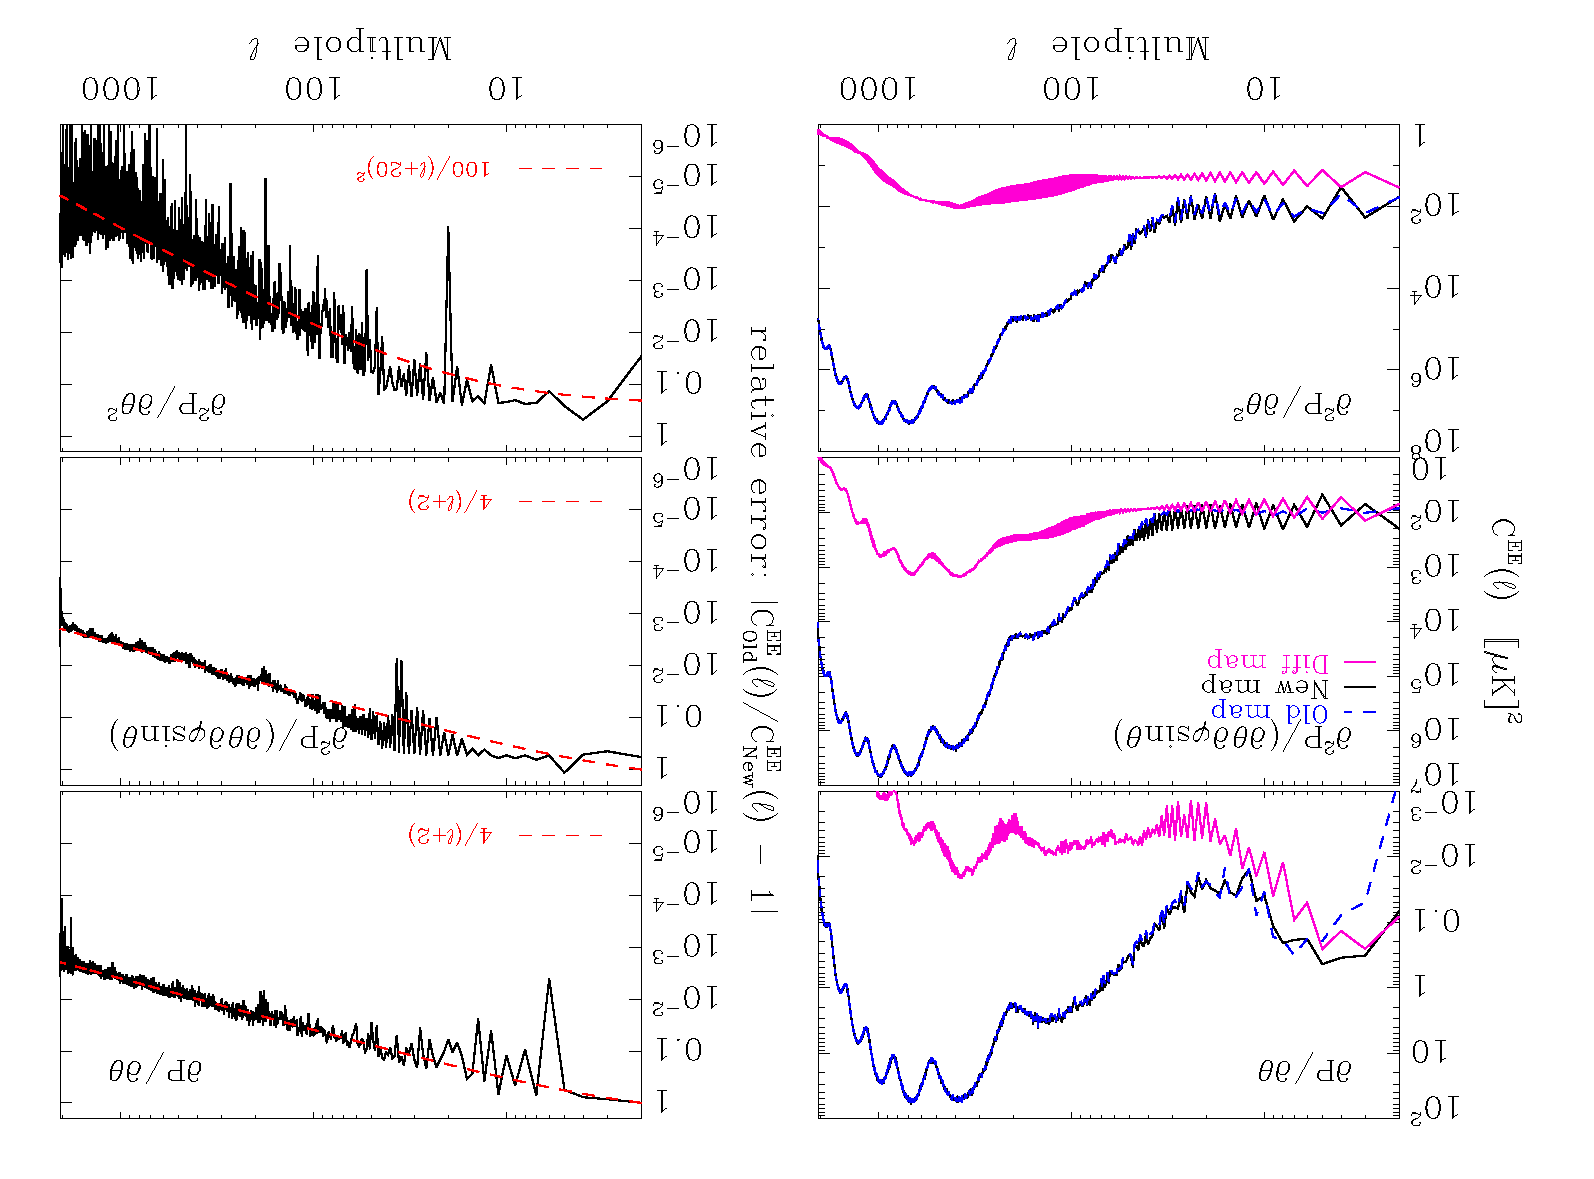
\includegraphics[width=0.99\textwidth,angle=-180]{fig/error_der.pdf}
% }{%for html
% \centerline{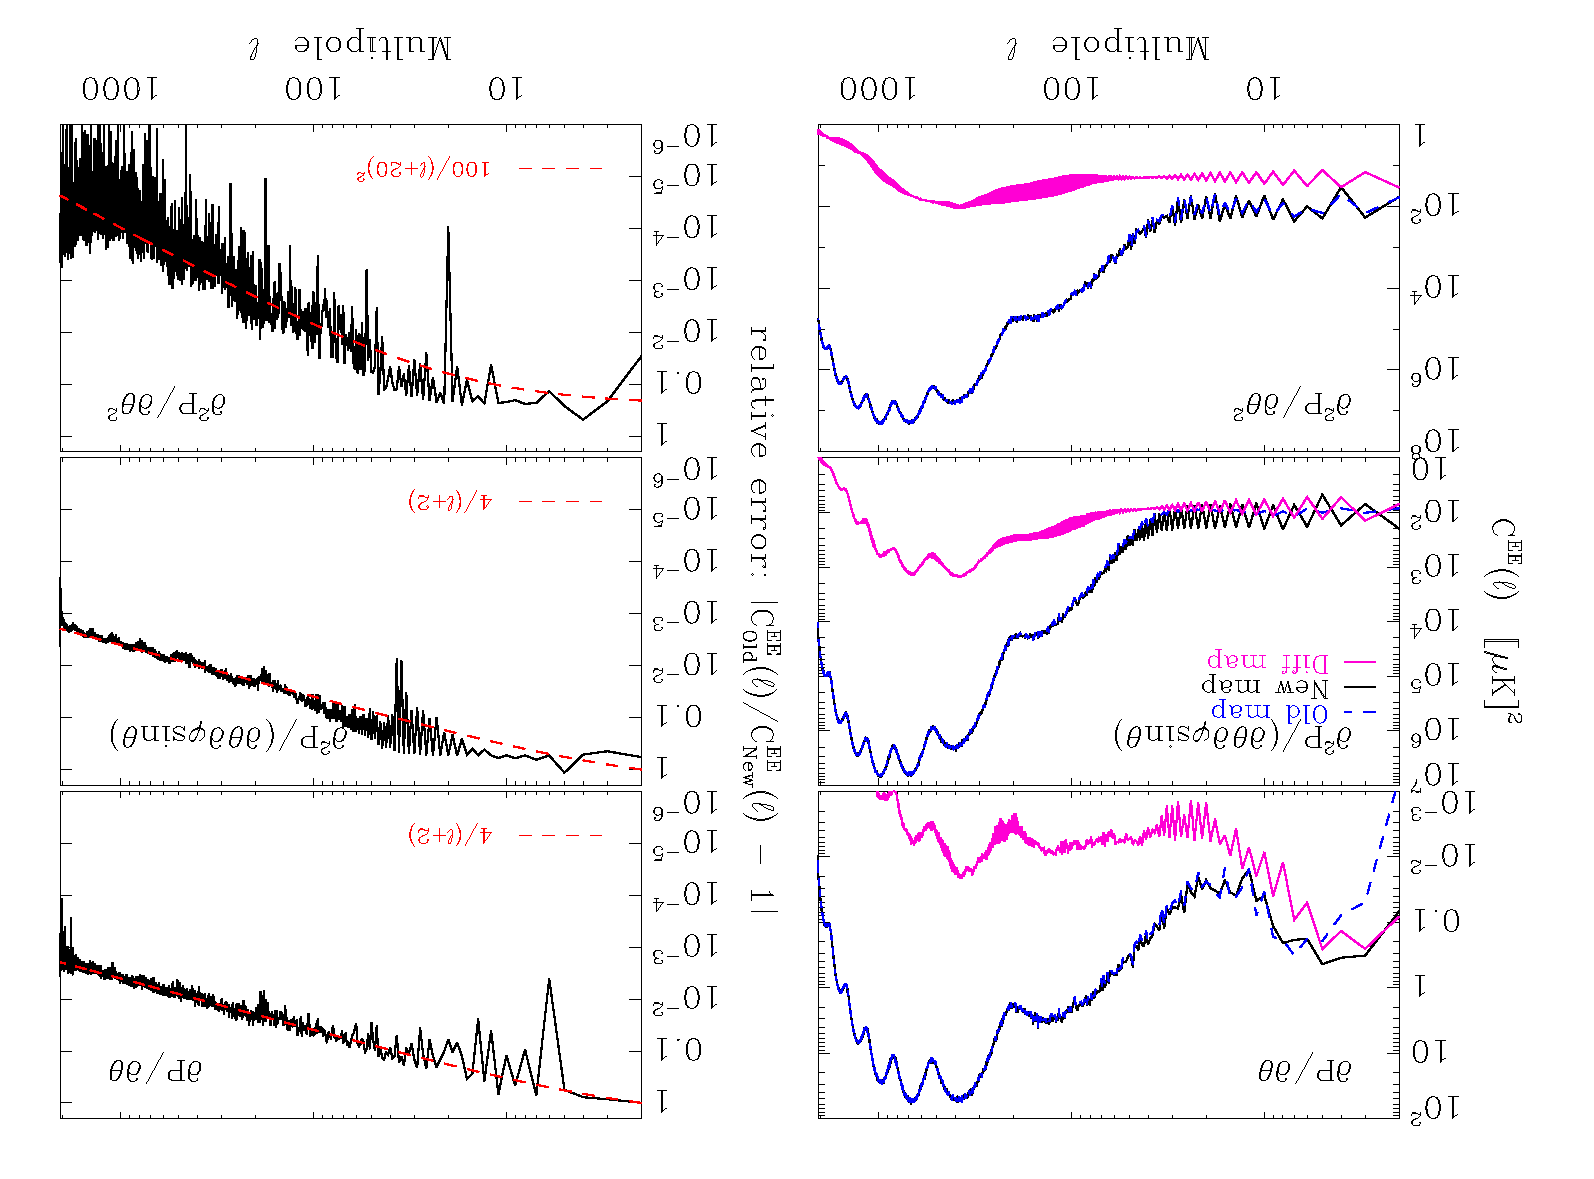
\includegraphics[width=520pt,angle=-180]{fig/error_der}}
% }
\latexhtml{%for latex
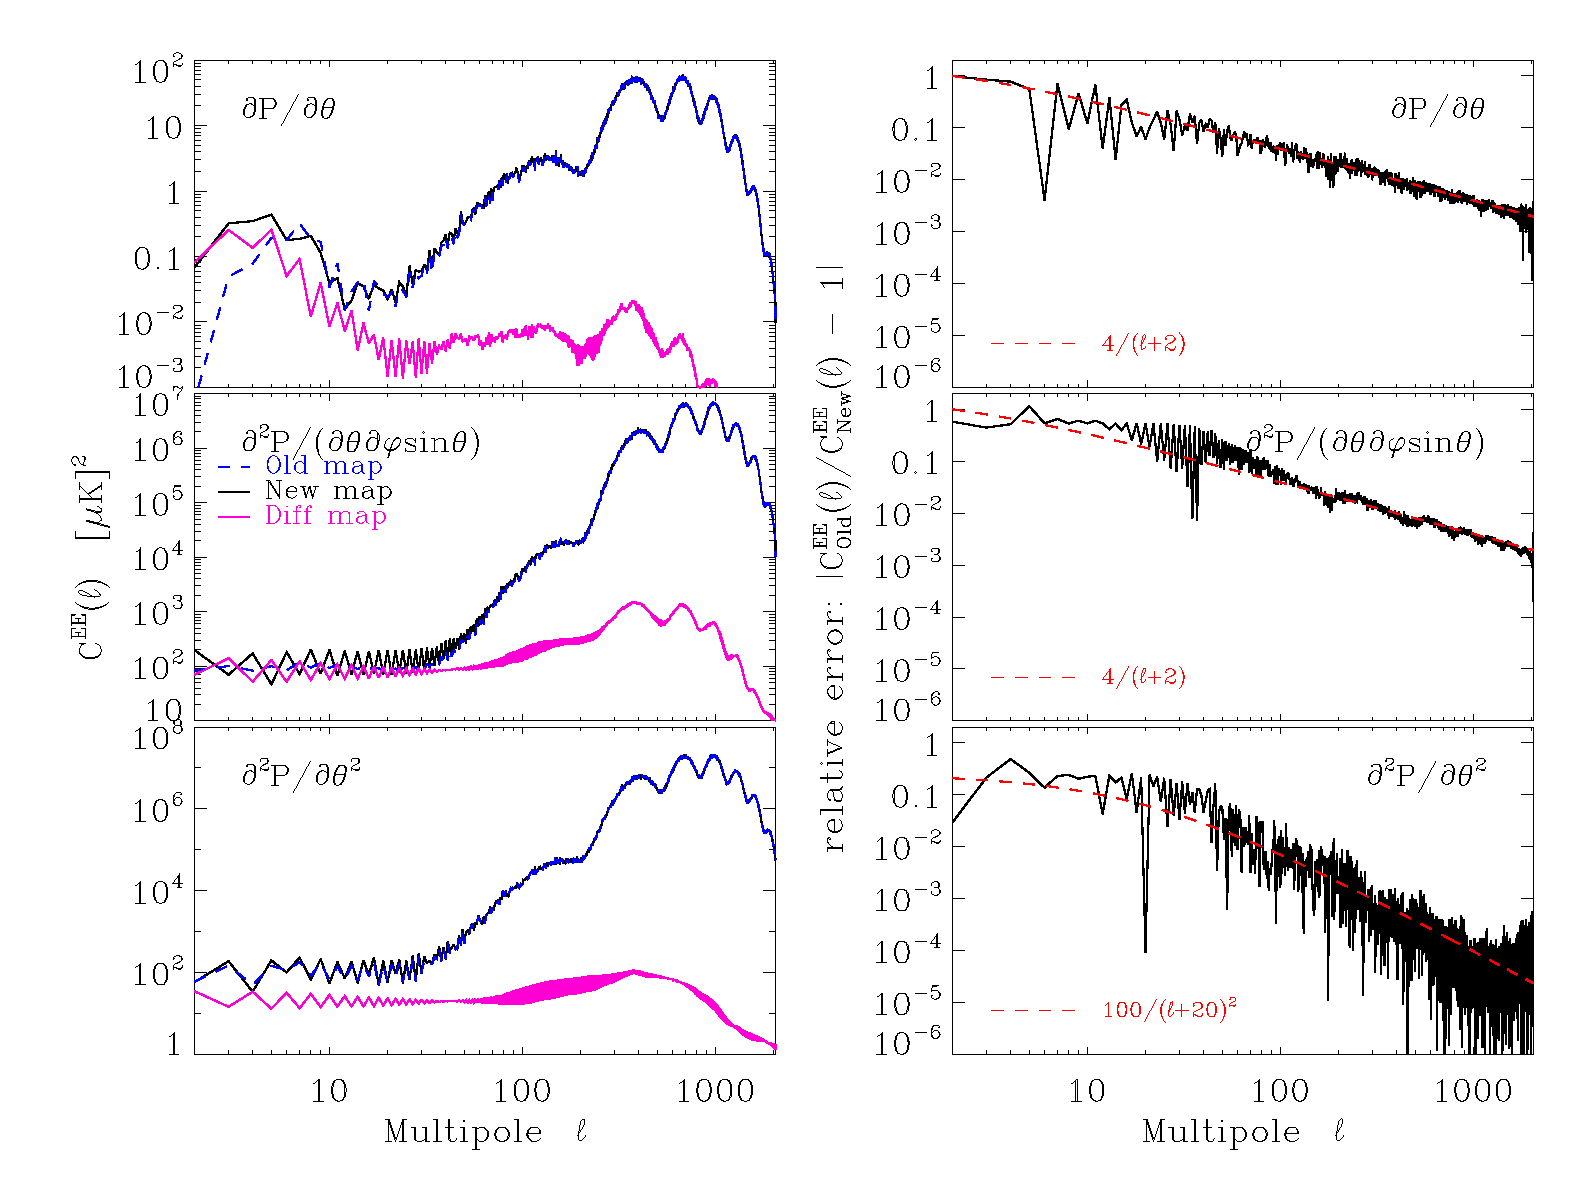
\includegraphics[width=0.99\textwidth]{fig/error_der_r180.pdf}
}{%for html
\centerline{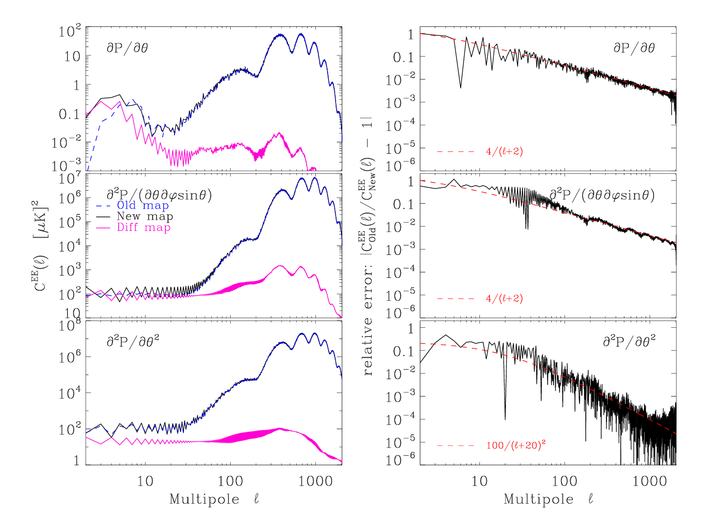
\includegraphics[width=520pt]{fig/error_der_r180}}
}
\caption[Derivatives power spectra]{%
\label{fig:bug_derQU}\latexhtml{\footnotesize}{}%
Left panels: comparison of the EE power spectra $C(\ell)$ computed on polarized maps
derivatives generated by
{\tt synfast}-2.13a (Old maps, blue bashes), the bug corrected {\tt synfast}-2.14 (New maps, black lines)
and their differences (Diff maps, magenta lines). Note that what is plotted is
$C(\ell)$, {\em not} the customary $\ell(\ell+1)C(\ell)/2\pi$. Right panels show respectively
the relative error on the EE power spectrum of the old derivatives maps compared
to that of the new maps.
The red dashes show analytical fit to these errors.
}
\end{figure}
%-----------------------------------------------------
In Figure~\ref{fig:bug_derQU} we show the polarization $EE$ power spectrum of
$\nside = 1024$ maps
in which the Stokes parameters $(Q,U)$ have been replaced by, in turn, their derivatives
$\partial (Q,U)/\partial\theta$, 
$\partial^2 (Q,U)/\partial \theta^2$, 
$\partial^2 (Q,U)/(\partial\theta\partial\varphi\sin\theta)$, 
for maps generated
by either the version 2.13a of {\tt synfast} or the corrected version 2.14, or
the difference of the two set of maps.
The input power spectra were those of WMAP-1yr $\Lambda$-CDM best fit model with a Gaussian
beam FWHM of 10 arcmin. The power spectra were computed on the whole maps, except
for 12 pixels around each pole that were masked out, because they get very
bright in second order derivatives.

It can be seen that the relative effect of the computation error on the produced maps was
large at low $\ell$, at scales on which derivatives maps contain little power, but decreasing
steadily with $\ell$.


\vskip 1cm
It should be stressed that the following quantities were {\em not} affected by
the bug described above:
\begin{itemize}
\item the Stokes parameters themselves $(I,Q,U)$,
\item the intensity $I$ and all its derivatives,
\item the Laplacians $\Delta I, \Delta Q$ and $\Delta U$, with
$\Delta \equiv \left(
\frac{\partial^2}{\partial\theta^2}
+ \cot\theta\frac{\partial}{\partial\theta} + 
\frac{\partial^2}{\sin^2\theta\partial\varphi^2} 
\right)$.
\end{itemize}


\end{document}
